\documentclass[10pt,twocolumn,letterpaper]{article}

\usepackage{wacv}

%------------------------------------------------------------------------------
% needed for externalization of plots (no margins on individual pdfs)
\newcommand{\finalcopy}{\iccvfinalcopy}
%------------------------------------------------------------------------------
% FIGURES: CHOOSE ONE OPTION
%
% plots:       build standalone pdfs for figures, then use them
% plots-ext:   use existing pdfs for figures
% plots-none:  skip figures
% 
%------------------------------------------------------------------------------
% hack for CVPR/ICCV style
\makeatletter
\@namedef{ver@everyshi.sty}{}
\makeatother

%------------------------------------------------------------------------------
% main packages
%\usepackage[dvipsnames,svgnames,x11names]{xcolor}
\usepackage{tikz}
\usetikzlibrary{arrows.meta,shapes,calc,matrix,fit,positioning,backgrounds,decorations.markings,fadings}
\usepackage{pgfplots}
\usepackage{pgfplotstable}
\usepgfplotslibrary{dateplot}
\pgfplotsset{compat=1.9}
\usepackage{xstring}

%------------------------------------------------------------------------------
% externalization: requires defining \finalcopy first

\usepgfplotslibrary{external}
% \tikzexternalize[prefix=fig/extern/]
\newcommand{\extfig}[2]{\tikzsetnextfilename{#1}{#2}}
\newcommand{\noextfig}[1]{\tikzset{external/export next={false}}{#1}}
\newcommand{\extdata}[1]{\input{#1}}
\IfBeginWith*{\jobname}{fig/extern/}{\finalcopy}{}

%-----------------------------------------------------------------------------
% tikz styles

\tikzstyle{every picture}+=[
	remember picture,
	every text node part/.style={align=center},
	every matrix/.append style={ampersand replacement=\&},
]
\tikzstyle{tight} = [inner sep=0pt,outer sep=0pt]
\tikzstyle{node}  = [draw,circle,tight,minimum size=12pt,anchor=center]
\tikzstyle{op}    = [draw,circle,tight]
\tikzstyle{dot}   = [fill,draw,circle,inner sep=1pt,outer sep=0]
\tikzstyle{pt}    = [fill,draw,circle,inner sep=1.5pt,outer sep=.2pt]
\tikzstyle{box}   = [draw,rectangle,inner sep=3pt]
\tikzstyle{high}  = [black!60]
\tikzstyle{group} = [high,box,opacity=.5]
\tikzstyle{dim1}  = [fill opacity=.3,text opacity=1]
\tikzstyle{dim2}  = [fill opacity=.5,text opacity=1]
\tikzstyle{dim3}  = [fill opacity=.7,text opacity=1]
\tikzstyle{rectc} = [tight,transform shape]
\tikzstyle{rect}  = [rectc,anchor=south west]

%-----------------------------------------------------------------------------
% framed figures

\newcommand{\framed}[3][1]{\extfig{#2}{\tikz{
	\node[tight](a){\fig[#1]{#3}};
	\node[tight,draw=gray,fit=(a)]{};
}}}

%-----------------------------------------------------------------------------
% pgfplots general options

\newcommand{\leg}[1]{\addlegendentry{#1}}

\tikzset{every mark/.append style={solid}}
\pgfplotsset{%smooth,
	grid=both, width=\columnwidth, try min ticks=5,
	every axis/.append style={font=\small},
	every axis plot/.append style={thick,mark=none,mark size=1.8,tension=0.18},
	legend cell align=left, legend style={fill opacity=0.8},
	xticklabel={\pgfmathprintnumber[assume math mode=true]{\tick}},
	yticklabel={\pgfmathprintnumber[assume math mode=true]{\tick}},
	nodes near coords math/.style={
	nodes near coords={\pgfmathprintnumber[assume math mode=true]{\pgfplotspointmeta}},
	},
}

\pgfplotsset{
	dash/.style={mark=o,dashed,opacity=0.6},
	dott/.style={mark=o,dotted,opacity=0.6},
	nolim/.style={enlargelimits=false},
	plain/.style={every axis plot/.append style={},nolim,grid=none},
}
%\pgfplotsset{scaled y ticks = false}
\newcommand{\kilo}[1]{\thisrow{#1}/1000}

%--------------------------------------------------------------------

% layers
\pgfdeclarelayer{bg4}
\pgfdeclarelayer{bg3}
\pgfdeclarelayer{bg2}
\pgfdeclarelayer{bg1}
\pgfdeclarelayer{fg1}
\pgfdeclarelayer{fg2}
\pgfdeclarelayer{fg3}
\pgfdeclarelayer{fg4}
\pgfsetlayers{bg4,bg3,bg2,bg1,main,fg1,fg2,fg3,fg4}

%------------------------------------------------------------------------------
% 3d drawing

\pgfkeys{/tikz/.cd, aspect/.store in=\aspect, aspect=1}
\pgfkeys{/tikz/.cd, depth/.store in=\depth, depth=.5}
\pgfkeys{/tikz/.cd, stepx/.store in=\step, stepx=1}

\tikzstyle{geom} = [line join=bevel,aspect=1,depth=.5,z={(\depth*\aspect,\depth)}]
\tikzstyle{wire} = [geom,draw,thick]

% 3d coordinates
\def\cx[#1,#2,#3]{#1}
\def\cy[#1,#2,#3]{#2}
\def\cz[#1,#2,#3]{#3}
\def\ex[#1,#2,#3]{#1,0,0}
\def\ey[#1,#2,#3]{0,#2,0}
\def\ez[#1,#2,#3]{0,0,#3}

% lines along x, y, or z
\newcommand{\zline}[3][]{%
\path[geom,#1] #2 -- +(\cx[#3],\cy[#3]);
}
\newcommand{\yline}[3][]{%
\path[geom,#1,shift={#2},xslant=\aspect]
	(0,0) -- +(\cx[#3],\depth*\cz[#3]);
}
\newcommand{\xline}[3][]{%
\path[geom,#1,shift={#2},yslant=1/\aspect]
	(0,0) -- +(\aspect*\depth*\cz[#3],\cy[#3]);
}

% rectangles / grids along x, y, or z
\newcommand{\zrect}[3][]{%
\path[geom,#1] #2 rectangle +(\cx[#3],\cy[#3]);
}
\newcommand{\yrect}[3][]{%
\path[geom,#1,shift={#2},xslant=\aspect]
	(0,0) rectangle +(\cx[#3],\depth*\cz[#3]);
}
\newcommand{\xrect}[3][]{%
\path[geom,#1,shift={#2},yslant=1/\aspect]
	(0,0) rectangle +(\aspect*\depth*\cz[#3],\cy[#3]);
}
\newcommand{\xgrid}[3][]{%
\path[geom,#1,shift={#2},yslant=1/\aspect,xstep=\aspect*\depth*\step]
	(0,0) grid +(\aspect*\depth*\cz[#3],\cy[#3]);
}

% parallepiped
\newcommand{\para}[4][]{%
\zrect[#1]{(#3)}{#4}                 % front
\yrect[#1]{($(#3)+(\ey[#4])$)}{#4}   % top
\xrect[#1]{($(#3)+(\ex[#4])$)}{#4}   % right
\path[geom]
	(#3) coordinate(#2-southwest)
	($(#3)+(#4)$) coordinate(#2-northeast)
	($(#3)+(\ey[#4])$) coordinate(#2-northwest)
	($(#3)+(#4)-(\ey[#4])$) coordinate(#2-southeast)
	($(#3)+.5*(\ex[#4])$) coordinate(#2-south)
	($(#3)+(#4)-.5*(\ex[#4])$) coordinate(#2-north)
	($(#3)+.5*(\ex[#4])+.5*(#4)$) coordinate(#2-center)
	(#2-southwest |- #2-center) coordinate(#2-west)
	(#2-center -| #2-northeast) coordinate(#2-east)
	;
}

% %------------------------------------------------------------------------------
% hack for CVPR/ICCV style
\makeatletter
\@namedef{ver@everyshi.sty}{}
\makeatother

%------------------------------------------------------------------------------
% main packages
\usepackage[dvipsnames,svgnames,x11names]{xcolor}
\usepackage{tikzextern}
\usepackage{pgffor}

%------------------------------------------------------------------------------
% externalization
\newcommand{\extfig}[2]{\tikzsetnextfilename{fig/extern/#1}{#2}}
\newcommand{\noextfig}[1]{!!!}
\newcommand{\extdata}[1]{}

% \newcommand{\extfig}[2]{!!!}
\newcommand{\noextfig}[1]{!!!}
\newcommand{\extdata}[1]{}

%------------------------------------------------------------------------------
% space before \paragraph (default 4.05ex)
\makeatletter
\renewcommand\paragraph{\@startsection{paragraph}{4}{\z@}{1ex}{-1em}{\normalfont\normalsize\bfseries}}
\makeatother
%------------------------------------------------------------------------------

\usepackage{times}
\usepackage{epsfig}
\usepackage{graphicx}
\usepackage{amsmath}
\usepackage{amssymb}

% Include other packages here, before hyperref.

\usepackage{float}
\usepackage{multirow}
\usepackage[numbers]{natbib}
\usepackage{enumitem}
\usepackage{array,booktabs}
\usepackage{bbm}
\usepackage{colortbl}


% If you comment hyperref and then uncomment it, you should delete
% egpaper.aux before re-running latex.  (Or just hit 'q' on the first latex
% run, let it finish, and you should be clear).
\usepackage[pagebackref=true,breaklinks=true,letterpaper=true,colorlinks,bookmarks=false]{hyperref}

% \iccvfinalcopy % *** Uncomment this line for the final submission

\def\wacvPaperID{140} % *** Enter the ICCV Paper ID here
\def\httilde{\mbox{\tt\raisebox{-.5ex}{\symbol{126}}}}

% Pages are numbered in submission mode, and unnumbered in camera-ready
\ifwacvfinal\pagestyle{empty}\fi

\begin{document}


\newcommand{\head}[1]{{\smallskip\noindent\textbf{#1}}}
\newcommand{\alert}[1]{{\color{red}{#1}}}
\newcommand{\sm}{\scriptsize}
\newcommand{\eq}[1]{(\ref{eq:#1})}

\newcommand{\Th}[1]{\textsc{#1}}
\newcommand{\mr}[2]{\multirow{#1}{*}{#2}}
\newcommand{\mc}[2]{\multicolumn{#1}{c}{#2}}
\newcommand{\tb}[1]{\textbf{#1}}
\newcommand{\ch}{\checkmark}

\newcommand{\red}[1]{{\color{red}{#1}}}
\newcommand{\blue}[1]{{\color{blue}{#1}}}
\newcommand{\green}[1]{{\color{green}{#1}}}
\newcommand{\gray}[1]{{\color{gray}{#1}}}

\newcommand{\citeme}[1]{\red{[XX]}}
\newcommand{\refme}[1]{\red{(XX)}}

\newcommand{\fig}[2][1]{\includegraphics[width=#1\linewidth]{fig/#2}}
\newcommand{\figh}[2][1]{\includegraphics[height=#1\linewidth]{fig/#2}}


\newcommand{\tran}{^\top}
\newcommand{\mtran}{^{-\top}}
\newcommand{\zcol}{\mathbf{0}}
\newcommand{\zrow}{\zcol\tran}

\newcommand{\ind}{\mathbbm{1}}
\newcommand{\expect}{\mathbb{E}}
\newcommand{\nat}{\mathbb{N}}
\newcommand{\zahl}{\mathbb{Z}}
\newcommand{\real}{\mathbb{R}}
\newcommand{\proj}{\mathbb{P}}
\newcommand{\prob}{\operatorname{P}}
\newcommand{\normal}{\mathcal{N}}

\newcommand{\mif}{\textrm{if}\ }
\newcommand{\other}{\textrm{otherwise}}
\newcommand{\minimize}{\textrm{minimize}\ }
\newcommand{\maximize}{\textrm{maximize}\ }
\newcommand{\st}{\textrm{subject\ to}\ }

\newcommand{\id}{\operatorname{id}}
\newcommand{\const}{\operatorname{const}}
\newcommand{\sgn}{\operatorname{sgn}}
\newcommand{\var}{\operatorname{Var}}
\newcommand{\mean}{\operatorname{mean}}
\newcommand{\trace}{\operatorname{tr}}
\newcommand{\diag}{\operatorname{diag}}
\newcommand{\vect}{\operatorname{vec}}
\newcommand{\cov}{\operatorname{cov}}
\newcommand{\sign}{\operatorname{sign}}
\newcommand{\prj}{\operatorname{proj}}

\newcommand{\softmax}{\operatorname{softmax}}
\newcommand{\clip}{\operatorname{clip}}

\newcommand{\defn}{\mathrel{:=}}
\newcommand{\peq}{\mathrel{+\!=}}
\newcommand{\meq}{\mathrel{-\!=}}

\newcommand{\floor}[1]{\left\lfloor{#1}\right\rfloor}
\newcommand{\ceil}[1]{\left\lceil{#1}\right\rceil}
\newcommand{\inner}[1]{\left\langle{#1}\right\rangle}
\newcommand{\norm}[1]{\left\|{#1}\right\|}
\newcommand{\abs}[1]{\left|{#1}\right|}
\newcommand{\frob}[1]{\norm{#1}_F}
\newcommand{\card}[1]{\left|{#1}\right|\xspace}

\newcommand{\diff}{\mathrm{d}}
\newcommand{\der}[3][]{\frac{\diff^{#1}#2}{\diff#3^{#1}}}
\newcommand{\ider}[3][]{\diff^{#1}#2/\diff#3^{#1}}
\newcommand{\pder}[3][]{\frac{\partial^{#1}{#2}}{\partial{{#3}^{#1}}}}
\newcommand{\ipder}[3][]{\partial^{#1}{#2}/\partial{#3^{#1}}}
\newcommand{\dder}[3]{\frac{\partial^2{#1}}{\partial{#2}\partial{#3}}}

\newcommand{\wb}[1]{\overline{#1}}
\newcommand{\wt}[1]{\widetilde{#1}}

\def\xssp{\hspace{1pt}}
\def\ssp{\hspace{3pt}}
\def\msp{\hspace{5pt}}
\def\lsp{\hspace{12pt}}

\newcommand{\cA}{\mathcal{A}}
\newcommand{\cB}{\mathcal{B}}
\newcommand{\cC}{\mathcal{C}}
\newcommand{\cD}{\mathcal{D}}
\newcommand{\cE}{\mathcal{E}}
\newcommand{\cF}{\mathcal{F}}
\newcommand{\cG}{\mathcal{G}}
\newcommand{\cH}{\mathcal{H}}
\newcommand{\cI}{\mathcal{I}}
\newcommand{\cJ}{\mathcal{J}}
\newcommand{\cK}{\mathcal{K}}
\newcommand{\cL}{\mathcal{L}}
\newcommand{\cM}{\mathcal{M}}
\newcommand{\cN}{\mathcal{N}}
\newcommand{\cO}{\mathcal{O}}
\newcommand{\cP}{\mathcal{P}}
\newcommand{\cQ}{\mathcal{Q}}
\newcommand{\cR}{\mathcal{R}}
\newcommand{\cS}{\mathcal{S}}
\newcommand{\cT}{\mathcal{T}}
\newcommand{\cU}{\mathcal{U}}
\newcommand{\cV}{\mathcal{V}}
\newcommand{\cW}{\mathcal{W}}
\newcommand{\cX}{\mathcal{X}}
\newcommand{\cY}{\mathcal{Y}}
\newcommand{\cZ}{\mathcal{Z}}

\newcommand{\vA}{\mathbf{A}}
\newcommand{\vB}{\mathbf{B}}
\newcommand{\vC}{\mathbf{C}}
\newcommand{\vD}{\mathbf{D}}
\newcommand{\vE}{\mathbf{E}}
\newcommand{\vF}{\mathbf{F}}
\newcommand{\vG}{\mathbf{G}}
\newcommand{\vH}{\mathbf{H}}
\newcommand{\vI}{\mathbf{I}}
\newcommand{\vJ}{\mathbf{J}}
\newcommand{\vK}{\mathbf{K}}
\newcommand{\vL}{\mathbf{L}}
\newcommand{\vM}{\mathbf{M}}
\newcommand{\vN}{\mathbf{N}}
\newcommand{\vO}{\mathbf{O}}
\newcommand{\vP}{\mathbf{P}}
\newcommand{\vQ}{\mathbf{Q}}
\newcommand{\vR}{\mathbf{R}}
\newcommand{\vS}{\mathbf{S}}
\newcommand{\vT}{\mathbf{T}}
\newcommand{\vU}{\mathbf{U}}
\newcommand{\vV}{\mathbf{V}}
\newcommand{\vW}{\mathbf{W}}
\newcommand{\vX}{\mathbf{X}}
\newcommand{\vY}{\mathbf{Y}}
\newcommand{\vZ}{\mathbf{Z}}

\newcommand{\va}{\mathbf{a}}
\newcommand{\vb}{\mathbf{b}}
\newcommand{\vc}{\mathbf{c}}
\newcommand{\vd}{\mathbf{d}}
\newcommand{\ve}{\mathbf{e}}
\newcommand{\vf}{\mathbf{f}}
\newcommand{\vg}{\mathbf{g}}
\newcommand{\vh}{\mathbf{h}}
\newcommand{\vi}{\mathbf{i}}
\newcommand{\vj}{\mathbf{j}}
\newcommand{\vk}{\mathbf{k}}
\newcommand{\vl}{\mathbf{l}}
\newcommand{\vm}{\mathbf{m}}
\newcommand{\vn}{\mathbf{n}}
\newcommand{\vo}{\mathbf{o}}
\newcommand{\vp}{\mathbf{p}}
\newcommand{\vq}{\mathbf{q}}
\newcommand{\vr}{\mathbf{r}}
\newcommand{\Vs}{\mathbf{s}}
\newcommand{\vt}{\mathbf{t}}
\newcommand{\vu}{\mathbf{u}}
\newcommand{\vv}{\mathbf{v}}
\newcommand{\vw}{\mathbf{w}}
\newcommand{\vx}{\mathbf{x}}
\newcommand{\vy}{\mathbf{y}}
\newcommand{\vz}{\mathbf{z}}

\newcommand{\vone}{\mathbf{1}}
\newcommand{\vzero}{\mathbf{0}}

\newcommand{\valpha}{{\boldsymbol{\alpha}}}
\newcommand{\vbeta}{{\boldsymbol{\beta}}}
\newcommand{\vgamma}{{\boldsymbol{\gamma}}}
\newcommand{\vdelta}{{\boldsymbol{\delta}}}
\newcommand{\vepsilon}{{\boldsymbol{\epsilon}}}
\newcommand{\vzeta}{{\boldsymbol{\zeta}}}
\newcommand{\veta}{{\boldsymbol{\eta}}}
\newcommand{\vtheta}{{\boldsymbol{\theta}}}
\newcommand{\viota}{{\boldsymbol{\iota}}}
\newcommand{\vkappa}{{\boldsymbol{\kappa}}}
\newcommand{\vlambda}{{\boldsymbol{\lambda}}}
\newcommand{\vmu}{{\boldsymbol{\mu}}}
\newcommand{\vnu}{{\boldsymbol{\nu}}}
\newcommand{\vxi}{{\boldsymbol{\xi}}}
\newcommand{\vomikron}{{\boldsymbol{\omikron}}}
\newcommand{\vpi}{{\boldsymbol{\pi}}}
\newcommand{\vrho}{{\boldsymbol{\rho}}}
\newcommand{\vsigma}{{\boldsymbol{\sigma}}}
\newcommand{\vtau}{{\boldsymbol{\tau}}}
\newcommand{\vupsilon}{{\boldsymbol{\upsilon}}}
\newcommand{\vphi}{{\boldsymbol{\phi}}}
\newcommand{\vchi}{{\boldsymbol{\chi}}}
\newcommand{\vpsi}{{\boldsymbol{\psi}}}
\newcommand{\vomega}{{\boldsymbol{\omega}}}

\newcommand{\rLambda}{\mathrm{\Lambda}}
\newcommand{\rSigma}{\mathrm{\Sigma}}

\newcommand{\vLambda}{\bm{\rLambda}}
\newcommand{\vSigma}{\bm{\rSigma}}

\makeatletter
\newcommand*\bdot{\mathpalette\bdot@{.7}}
\newcommand*\bdot@[2]{\mathbin{\vcenter{\hbox{\scalebox{#2}{$\m@th#1\bullet$}}}}}
\makeatother

\makeatletter
\DeclareRobustCommand\onedot{\futurelet\@let@token\@onedot}
\def\@onedot{\ifx\@let@token.\else.\null\fi\xspace}

\def\eg{\emph{e.g}\onedot} \def\Eg{\emph{E.g}\onedot}
\def\ie{\emph{i.e}\onedot} \def\Ie{\emph{I.e}\onedot}
\def\cf{\emph{cf}\onedot} \def\Cf{\emph{Cf}\onedot}
\def\etc{\emph{etc}\onedot} \def\vs{\emph{vs}\onedot}
\def\wrt{w.r.t\onedot} \def\dof{d.o.f\onedot} \def\aka{a.k.a\onedot}
\def\etal{\emph{et al}\onedot}
\makeatother

\newcommand{\relu}{\operatorname{ReLU}}
\newcommand{\gap}{\operatorname{GAP}}
\newcommand{\up}{\operatorname{Up}}
\newcommand{\ce}{\operatorname{CE}}

\newcommand{\cam}{\textrm{CAM}}
\newcommand{\gcam}{\textrm{Grad-CAM}}
\newcommand{\scam}{\textrm{Score-CAM}}

\newcommand{\mae}{\textrm{MAE}}
\newcommand{\mse}{\textrm{MSE}}
\newcommand{\hi}{\textrm{HI}}


%%%%%%%%% TITLE
\title{\Ours: Attention based pooling for interpretable image recognition}

\author{First Author\\
Institution1\\
Institution1 address\\
{\tt\small firstauthor@i1.org}
% For a paper whose authors are all at the same institution,
% omit the following lines up until the closing ``}''.
% Additional authors and addresses can be added with ``\and'',
% just like the second author.
% To save space, use either the email address or home page, not both
\and
Second Author\\
Institution2\\
First line of institution2 address\\
{\tt\small secondauthor@i2.org}
}

\maketitle
% Remove page # from the first page of camera-ready.
\ifwacvfinal\thispagestyle{empty}\fi


%%%%%%%%% ABSTRACT
\begin{abstract}
The recent introduction of Visual Transformers, performing image recognition tasks, reduce the attention given to Convolutional Neural Networks (CNNs). One of the key factors leading to this transition is the difference between building blocks of Visual Transformers and CNNs; where the former makes use of the self attention mechanism which is a global operation, and the latter relying upon convolution operations, which are mostly local.\\
In this work we introduce CLS-Pooling, incorporating ideas from visual transformers into CNNs. Our approach consists of a cross-attention based stream that can be attached alongside CNN architectures to improve their interpretability properties and their recognition capabilities. We observe that this approach improves the classification properties of several standard CNNs while maintaining or improving their explainability properties.
\end{abstract}

%%%%%%%%% BODY TEXT
%--------------------------------------------------------------------------------------------------
\addchap{Introduction}
%\addcontentsline{toc}{chapter}{Introduction}
\noindent Amongst the sensory information that the brain processes, visual stimuli accounts 
for 90\% of data analyzed \autocite{potter2014detecting}, while consuming a great amount of energy 
in human metabolism (\cite{phelps1981metabolic}). It is argued that a big influence on the 
brain evolution was as a result of improving the capacity to process this kind of data and the 
ensuing  pattern recognition (\cite{mattson2014superior}). 
Currently, these shapes and forms have evolved too: it is no longer common for a human in most 
metropolitan areas, the need to scan the environment for faces that could reveal a potential 
predator; for a change, the patterns that we now seek to unravel also contain products of our own 
imagination: digits and characters, geometrical shapes.\\

\paragraph{Visual Recognition} Understanding the processes behind visual recognition has been a 
prominent research question throughout human history. From the preliminary questionings by greek  
philosphers (\cite{finger2001origins}) to physics based studies like those by Newton and Locke 
(\cite{swenson2010optics}), and more recently with theories like \textit{Unconscious Inference} 
(\cite{gullstrand1909hemholtz}) and \textit{Gestalt} (\cite{wagemans2012century}), many proposals 
to understand and describe this process have been brought forth. Moreover, vision recogniton is not 
only studied in fields like physics, medicine and psychology; 
with the advent of computer science, computational approaches and theories started emerging 
regarding this domain. One such study that proved seminal in this domain is that carried out by 
David Marr (\cite{poggio1981marr}, \cite{marr2010vision}). Most notably, Marr addressed vision on 
three levels: comptational, algorithmic and implementation. In particular, upon the computational 
level, Marr pondered around issues that the visual system answers and their explanation; this 
ultimately led to the formulation of fundamental tasks within computer vision such as object 
recognition and reconstruction. Over the past decade great advancements were made on computer 
vision. In particular with the optimization and popularization of \gls{gpu}, models requiring 
a strong computational power became accesible for researchers. To be specific, the framework 
developed by Yann LeCun (\cite{lecun1998gradient}) got revitalized in 2012 with the introduction of 
AlexNet (\cite{krizhevsky2012imagenet}) where proper leverage of these machines outclassed that of 
more traditional machine learning models, Chapter \ref{ch:rel} discusses this in more depth. 
In this short span of time, several groundbreaking architectures have been proposed, in 
particular the ResNet family (\cite{he2016deep}) has remained relevant given its properties
(\cite{wightman2021resnet}); furthermore, with the introduction of the transformer architecture 
(\cite{vaswani2017attention}) this field of research recieved a new impulse and more powerful 
models based upon its functional unit are being brought forth.\\

\noindent It is not only with the increase of computational power that computer vision has improved over time. 
With the developement, popularization and spread of the internet; large collections of data have been 
formed. These aggregations can be extremely specific for a given end, or 
quite general representing the common interests of its users. Over time, these compilations have 
continued to grow both in volume and variety; still, several curated collections are introduced by 
researchers to experiment and control the development of models such as MNIST (\cite{lecun1998gradient}),
BSDS (\cite{MartinFTM01}), Pascal VOC (\cite{pascal-voc-2012}) and most notably, 
ImageNet (\cite{ILSVRC15}) and MS-COCO (\cite{lin2014microsoft}). Additionally, data collection is
an ongoing and a never ending process; as such, the idea of a dataset containing all types of 
information is no longer deemded a dream but a reality that might come true aided by Big Data in 
the foreseeable future \autocite{chen2014big}.\\

\noindent Taking into consideration the aforementioned  increase on  both compute power and data 
availability, deep learning based models have been steadily adopted and assimiliated within society; 
nowadays its no longer so much a question \textit{whether can a model achieve a given task}, but 
rather a question on \textit{how can this given model perform this task}. Providing an answer to 
this question is paramount as human lives are now being directly affected by such kind of models. 
The main issue behind understanding deep models, lies within the size and complexity of deep 
architecttures, where providing interpretable explanations has lead to the surge of a novel field 
of research (\cite{guidotti2018survey}, \cite{bodria2021benchmarking}).

\paragraph{Interpretability}
To begin discussing about interpretability, one must ponder around its definition. 
Over the last decade, many authors have attempted to address to this question. One 
of the most notable discussions can be found within \emph{The Mythos of Model Interpretability} 
(\cite{mythos_interp}). In this work, Lipton argues that for a model to be interpretable it must 
display two properties, \emph{Transparency} and \emph{Post-Hoc Interpretability}. In one hand, 
\textit{Transparency} answers questions regarding the model structure, training and inference 
processes; while on another hand, \textit{Post-Hoc Interpretability} relates to the explanations 
and information that can be drawn of the model itself.

\noindent Considering these properties, we observe that as machine learning models grew in 
complexity; their transparent properties vanished proportionaly to their size. It can be argued 
that traditional models offer themselves to  transparency due to their straightforward formulation 
and inherent properties. Conversely, in terms of post-hoc interpretations, methods like decision 
trees \cite{breiman2017classification} can be pruned to study their performance by removing 
branches (\cite{lakkaraju2016interpretable},\cite{mothilal2020explaining}). 
On another hand, established techniques such as Principal Component Analysis \gls{pca} 
(\cite{wold1987principal}), can be used to gain insight within data leading to a prediction.\\

\noindent When studying deep models, we find that it is after their size and complexity that their 
interpretable propierties get hindered. Common Convolutional Neural Networks \glspl{cnn} 
rely convolution as their corner stone, coupled with non-linear operations such as 
ReLU (\cite{fukushima1975cognitron}), Sigmoid, and Softmax (\cite{hopfield1985neural}) among others.
This aggregation of convolutions on one hand enables these models to process large quantities of 
data, and to a certain extent generalize; however, it also results in an extensive parameter count,
often reaching of millions, and most recently, even billions (\cite{openai_compute}). The 
computational load required for inference, typically measured in \gls{gflops} further compounds 
complexity.\\

\noindent Among the properties proposed by Lipton, we observe that offering model transparency is a 
rather challenging task. While understanding the behaviour of convolutions and 
self-attention might seem straightforward, it is their aggregation and subsequent flow of information what 
makes this process intricate. Moreover, transparency encompases aspects related to both
inference and training. In this regard, while deep learning research is often seen as an open field;
complete transparency is often disregarded as some authors frequently omit key details in their 
descriptions and methodologies. 

In contrast to transparency, providing post-hoc interpretations from deep models is a 
thriving field, where many of the challenges found within transparency are no longer found.
Within this field, various approaches have been proposed to achieve post-hoc interpretability,
including input masking (\cite{petsiuk2018rise}), attribution generation (\cite{NIPS2017_7062}, 
\cite{zhou2016learning}) and model perturbations 
(\cite{fong2017interpretable}, \cite{fong2019understanding}). Furthermore, the development of 
evaluation methodologies for these approaches has continued in tandem with them 
(\cite{choe2020evaluating}, \cite{chattopadhay2018grad}). Chapter \ref{ch:rel} delves deeper into 
these works. 

\paragraph{Dissertation Outline}
%\addcontentsline{toc}{section}{Dissertation Outline}
\noindent This dissertation is organized in the following manner: In Chapter \ref{ch:rel} we 
introduce a background for image recognition models (Section \ref{rel:sec_imrecon}) and the ensuing 
approaches developed to study the interpretability on them (Section \ref{rel:sec_int}). 
Additionally, we introduce evaluation procedures for these approaches which will be further used to 
evaluate ourproposals.\\

\noindent In Chapter \ref{ch:opticam}, we propose Opti-CAM as a methodology that generates 
optimized saliency maps highlighting the relevant regions on an image towards image classification. 
In Section \ref{sec:av_gain} we extend existing evaluation metrics with a novel measurement for 
model coinfidence. 
In Sections \ref{sec:oc_qual} and \ref{sec:oc_quant} we evaluate the effect of these contributions 
towards interpretability assessment.\\

\noindent Chapter \ref{ch:castream} introduces the Cross Attention Stream, an approach that boosts existing 
architectures interpretable properties. We ste up the modulus of this approach in 
Section \ref{sec:ca_defn} alongside its deployment on Section \ref{sec:ca_design}. 
In Sections \ref{sec:ca_qual} and \ref{sec:ca_quant} we demonstrate the benefits of using this
proposal.\\

\noindent Chapter \ref{ch:grad} characterizes a gradient denoising approach with a gradient denoising 
methodology as an approach to enhance the trainining procedure of current models while improving 
interpretability properties. In Section \ref{sec:grad_defn}, we define the gradient denoising 
protocol alongside the regularization proposals to do so.
Sections \ref{sec:grad_qual} and \ref{sec:grad_quant} illustrate the effects of this paradigmn
in the trained models and its effects on interpretability.\\

\noindent Chapter \ref{ch:zip} raises the Zero-Information algorithm and its usage as a substitute
for mask-dependent evaluation proposals. Section \ref{sec:zip_algo} develops this 
method. Section \ref{sec:zip_insdel} demonstrates its incorporation of this 
algorithm onto evaluation protocols. Section \ref{sec:zip_qual} displays
the effect of this approach when applied to mask patches on images. Section 
\ref{sec:zip_benchmark} displays the results of benchmarking these protocols 
with this approach. \\
    
\noindent Finally, we draw conclusions on our work and detail future research perspectives.
\section{Related Work}

\subsection{Interpretability}

To open up the black-box behavior of deep neural networks, model interpretability is mainly investigated along two directions~\citep{lipton18, guidotti2018survey, zhang2021survey}:
\begin{enumerate}[itemsep=2pt, parsep=0pt, topsep=3pt]
	\item \emph{Post-hoc interpretability} considers the model as a black-box and provides explanations based on inputs and outputs, without modifying the model or its training process.
	\item \emph{Transparency} modifies the model or the training process to better explain the behavior of the inner parts of the model.
\end{enumerate}

\paragraph{Post-hoc interpretability}

Approaches can be grouped into a number of possibly overlapping categories. \emph{Gradient-based methods}~\citep{adebayo2018local, springenberg2014striving, baehrens2010explain, simonyan2013deep, smilkov2017smoothgrad, bach2015pixel, sundararajan2017axiomatic} use the gradient of a target class score with respect to the input to compute the contribution of different input regions to the prediction. \emph{CAM-based methods}~\citep{DBLP:journals/corr/abs-1910-01279, DBLP:journals/corr/abs-1710-11063, DBLP:journals/corr/SelvarajuDVCPB16, fu2020axiom, jiang2021layercam, ramaswamy2020ablation} compute saliency maps as a linear combination of feature maps, with different definitions for the weights. \emph{Occlusion or masking-based methods}~\citep{petsiuk2018rise, fong2017interpretable, fong2019understanding, schulz2020restricting, ribeiro2016should} apply a number of candidate masks in the input space, measure their effect on the prediction and then combine them into a saliency map. Masking in feature space has been explored too~\cite{schulz2020restricting}. Finally, \emph{learning-based methods}~\citep{chang2018explaining, dabkowski2017real, phang2020investigating, zolna2020classifier, schulz2020restricting} learn an additional network or branch on extra data to produce an explanation map for a given input. 

Our method shares similarities with learning-based methods. In particular, we train an additional branch on the same training data as the network we aim to explain, but we only use the standard classification loss and we do not provide any explanation as output. Our method is also similar to CAM-based and masking-based methods exactly because we show that attention-based pooling is the same as masking in the feature space with weights obtained by a CAM-based saliency map.

\paragraph{Transparency}

Approaches are grouped in a number of categories according to the type of the given explanation. \emph{Rule-based methods}~\citep{wu2018beyond, wu2020regional} train a decision tree as a surrogate regularization term to force a network to be easily approximated by a decision tree.
% or learn a set of logit rules as an explanation~\citep{azzolin2022global}.
\emph{Hidden semantics-based methods}~\citep{bau2017network, zhou2018interpreting, zhang2018interpretable, zhou2014object} aim to make a convolutional network learn disentangled hidden semantics with hierarchical structure or object-level concepts.
\emph{Prototype-based methods}~\citep{li2018deep, chen2019looks} learn a set of prototypes or parts as an intermediate representation in the network, which can be aligned with categories. \emph{Attribution-based methods}~\citep{ismail2021improving, Zhou_2022_BMVC, ross2017right, ghaeini2019saliency} usually modify the architecture of a network or the training process to help post-hoc methods produce better saliency maps. Unlike~\citep{ross2017right, ghaeini2019saliency}, saliency guided localization~\citep{Zhou_2022_BMVC} does not need ground truth explanations but replaces them with information bottleneck attribution~\citep{schulz2020restricting}. Finally, saliency-guided training~\citep{ismail2021improving} minimizes the KL divergence between the output of original and masked images.

Our method belongs to attribution-based methods. We introduce a learnable cross-attention stream into the network as a pooling mechanism to replace \gap. As a result, post-hoc attribution-based methods can provide a better explanation. Although the network is modified, the training process is not: the network and classifier are pretrained and kept frozen while we learn the paramaters of our stream.

%------------------------------------------------------------------------------

\subsection{Attention-based architectures}

Attention is a powerful mechanism that has been introduced into convolutional networks in several ocaasions~\citep{bello2019attention, ramachandran2019stand, shen2020global}. With the success of vision transformers (ViT)~\citep{dosovitskiy2020image}, fully attention-based architectures are now competitive with convolutional networks. To benefit from both self-attention and convolutional layers, some hybrid architectures employ convolutional layers before the vision transformer~\citep{graham2021levit,xiao2021early}. Others, such as Swin~\citep{liu2021swin} and PiT~\citep{heo2021rethinking}, introduce a pyramid structure to share local spatial information while reducing the spatial resolution, as in convolutional networks. 

Conformer~\citep{peng2021conformer} proposes a dual network structure to retrain and fuse local convolutional features with global representations. Our method merely provides a simple attention-based pooling mechanism inspired by transformers that can work with any architecture, even pretrained and frozen. SCOUTER~\citep{li2021scouter} uses slot attention~\cite{locatello2020object} to build a class specific pooling mechanism, which does not scale well to more than 20 classes. Our mechanism is based standard cross attention, it is class agnostic and scales up to 1000 classes, improving post-hoc interpretability without degrading classification accuracy. PatchConvNet~\citep{touvron2021augmenting} replaces global average pooling by an attention-based pooling layer. Our method is similar in this respect, but uses information collected from the entire network by a parallel processing stream. We introduce our mechanism into any convolutional network and study its effect on post-hoc interpretability.








\section{Opti-CAM}
\label{sec:opticam}

\subsection{Preliminaries}
\label{sec:prelim}

\paragraph{Notation}
\label{sec:notation}

Consider a classifier network $f: \cX \to \real^C$ that maps an input image $\vx \in \cX$ to a logit vector $\vy = f(\vx) \in \real^C$, where $\cX$ is the image space and $C$ is the number of classes. We denote by $y_c = f(\vx)_c$ the predicted logit and by $p_c = \softmax(\vy)_c \defn e^{y_c} / \sum_j e^{y_j}$ the predicted probability for class $c$. For layer $\ell$ with $K_\ell$ channels, we denote by $A^k_\ell = f^k_\ell(\vx) \in \real^{h_\ell \times w_\ell}$ the feature map for channel $k \in \{1,\dots,K_\ell\}$, with spatial resolution $h_\ell \times w_\ell$. Because of $\relu$ non-linearities, we assume that feature maps are non-negative. Similarly, we denote by $S_\ell \in \real^{h_\ell \times w_\ell}$ a 2D saliency map.

%------------------------------------------------------------------------------

\paragraph{Background: CAM-based saliency maps}
\label{sec:back}

Given a layer $\ell$ and a class of interest $c$, we consider saliency maps given by the general formula
\begin{equation}
	S^c_\ell(\vx) \defn h \left( \sum_k w^c_k A^k_\ell \right),
\label{eq:sal}
\end{equation}
where $w^c_k$ are weights defining a linear combination over channels and $h$ is an activation function. CAM~\citep{zhou2016learning} is defined for the last layer $L$ only with $h$ being the identity mapping and $w^c_k$ being the classifier weight connecting the $k$-th channel with class $c$. Grad-CAM~\citep{selvaraju2017grad} is defined for any layer $\ell$ with $h = \relu$ and weights
\begin{equation}
	w^c_k \defn \gap \left( \pder{y_c}{A^k_\ell} \right),
\label{eq:gcam}
\end{equation}
where $\gap$ is global average pooling.
% and $\softmax(\vy)_c = e^{y_c} / \sum_j e^{y_j}$ is the predicted probability of class $c$.
The motivation for $\relu$ is that we are only interested in features that have a positive effect on the class of interest, \ie pixels whose intensity should be increased in order to increase $y_c$.

Score-CAM~\cite{wang2020score} is also defined for any layer $\ell$ with $h = \relu$ and weights $w^c_k \defn \softmax(\vu^c)_k$.  Softmax normalization considers positive channel contributions only and attends to few feature maps.
%that \alert{produce less highlighted areas in the saliency map}. \iavr{Last part unclear.}
Here, vector $\vu^c \in \real^{K_\ell}$ measures the increase in confidence for class $c$ that compares a known baseline image $\vx_b$ with the input image $\vx$ masked according to feature map $A^k_\ell$, for all channels $k$:
\begin{equation}
	u^c_k \defn f(\vx \odot n(\up(A^k_\ell)))_c - f(\vx_b)_c,
\label{eq:s-cam}
\end{equation}
where $\odot$ is the Hadamard product. For this to work, the feature map $A^k_\ell$ is adapted to $\vx$ first: $\up$ denotes upsampling to the spatial resolution of $\vx$ and
\begin{equation}
	n(A) \defn \frac{A - \min A}{\max A - \min A}
\label{eq:norm}
\end{equation}
\redred{is a normalization of matrix $A$ into $[0,1]$.} While Score-CAM does not need gradients, it requires as many forward passes through the network as the number of channels in the chosen layer, which is computationally expensive.

%------------------------------------------------------------------------------

\paragraph{Motivation}
\label{sec:motiv}

\iavr{Score-CAM considers each feature map as a mask in isolation. How about linear combinations?} Given a vector $\vw \in \real^{K_\ell}$ with $w_k$ its $k$-th element, let
\begin{equation}
	F(\vw) \defn f \left( \vx \odot n \left( \up \left(
		\displaystyle\sum_k w_k A^k_\ell
	\right) \right) \right)_c.
\label{eq:s-obj}
\end{equation}
\ronan{If we assume that $\vx_b = \vzero$ in~\eq{s-cam} and define $n(\vzero) \defn \vzero$ in~\eq{norm}, then we can rewrite the right-hand side of~\eq{s-cam} as
\begin{equation}
	\frac{F(\vw_0 + \delta \ve_k) - F(\vw_0)}{\delta},
\label{eq:s-cam2}
\end{equation}
where $\vw_0 = \vzero$, $\delta = 1$ and $\ve_k$ is the $k$-th standard basis vector of $\real^{K_\ell}$. This resembles the numerical approximation of the derivative $\pder{F}{w_k}(\vw_0)$, except that $\delta$ is not small as usual. One could compute derivatives efficiently by standard backpropagation instead. It is then possible to iteratively optimize $F$ with respect to $\vw$, starting at any $\vw_0$.}

\iavr{As an alternative, consider masking-based methods relying on optimization in the input space, like \emph{meaningful perturbations} (MP)~\cite{fong2017interpretable} or \emph{extremal perturbations}~\citep{fong2019understanding}. In general, optimization takes the form
\begin{equation}
	S^c(\vx) \defn \arg\max_{\vm \in \cM} f(\vx \odot n(\up(\vm)))_c + \lambda R(\vm).
\label{eq:mask}
\end{equation}
Here, a mask $\vm$ is directly optimized and does not rely on feature maps, hence the saliency map $S^x(\vx)$ is not connected to any layer $\ell$. The mask is at the same or lower resolution than the input image. In the latter case, upsampling is still necessary.

In this approach, one indeed computes derivatives by backpropagation and indeed iteratively optimizes $\vm$. However, because $\vm$ is high-dimensional, there are constraints expressed by $\vm \in \cM$, \eg $\vm$ has a certain norm, and regularizers like $R(\vm)$, \eg $\vm$ is smooth in a certain way. This makes optimization harder or more expensive and introduces more hyperparameters like $\lambda$. One could simply constrain $\vm$ to lie in the linear span of $\{A_\ell^k\}_{k=1}^{K_\ell}$ instead, like all CAM-based methods.}

%------------------------------------------------------------------------------

\subsection{Method}
\label{sec:method}

\paragraph{Saliency maps}

As motivated by \autoref{sec:motiv}, we obtain a saliency map as a convex combination of feature maps by optimizing a given objective function with respect to the weights.
In particular, following~\citep{wang2020score}, we use channel weights $w_k \defn \softmax(\vu)_k$, where $\vu \in \real^{K_\ell}$ is a variable.
We then consider saliency map $S_\ell$ in layer $\ell$ as a function of both the input image $\vx$ and variable $\vu$:
\begin{equation}
    S_\ell(\vx; \vu) \defn \sum_k \softmax(\vu)_k A^k_\ell.
\label{eq:v-sal}
\end{equation}
Comparing with~\eq{sal}, $h$ is the identity mapping, because feature maps are non-negative and weights are positive.

%------------------------------------------------------------------------------

\paragraph{Optimization}

Now, given a layer $\ell$ and a class of interest $c$, we find the vector $\vu^*$ that maximizes the classifier confidence for class $c$, when the input image $\vx$ is masked according to saliency map $S_\ell(\vx; \vu^*)$:
\begin{equation}
	\vu^* \defn \arg\max_{\vu} F^c_\ell(\vx; \vu),
\label{eq:opt}
\end{equation}
where we define the objective function
\begin{equation}
	%F^c_\ell(\vx; \vu) \defn \abs{g_c(f(\vx \odot n(\up(S_\ell(\vx; \vu))))) - g_c(f(\vx))}.
	F^c_\ell(\vx; \vu) \defn g_c(f(\vx \odot n(\up(S_\ell(\vx; \vu))))).
\label{eq:obj}
\end{equation}
Here, the saliency map $S_\ell(\vx; \vu)$ is adapted to $\vx$ exactly as in~\eq{s-cam} in terms of resolution and normalization. For \emph{normalization function} $n$, the default is~\eq{norm}. The \emph{selector function} $g_c$ operates on the logit vector $\vy$; the default is to select the logit of class $c$, \ie $g_c(\vy) \defn y_c$. Other choices, including the definition of $F^c_\ell$ itself, are investigated in \autoref{sec:ablation} \redred{and in the supplementary material.}

%------------------------------------------------------------------------------

\paragraph{Opti-CAM}

Putting everything together, we define
\begin{equation}
	S^c_\ell(\vx) \defn S_\ell(\vx; \vu^*) = S_\ell(\vx; \arg\max_{\vu} F^c_\ell(\vx; \vu)),
\label{eq:o-sal}
\end{equation}
where $S_\ell$ and $F^c_\ell$ are defined by~\eq{v-sal} and~\eq{obj} respectively. The objective function $F^c_\ell$~\eq{obj} depends on variable $\vu$ through $S_\ell$~\eq{v-sal}, where the feature maps $A^k_\ell = f^k_\ell(\vx)$ are fixed. Then,~\eq{obj} involves masking and a forward pass through the network $f$, which is also fixed.

\autoref{fig:idea} is an abstract illustration of our method, \iavr{called Opti-CAM}, without details like upsampling and normalization~\eq{obj}. Optimization takes place along the highlighted path from variable $\vu$ to objective function $F^c_\ell$. The saliency map is real-valued and the entire objective function is differentiable in $\vu$. We use Adam optimizer~\citep{kingma2014adam} to solve the optimization problem~\eq{opt}.

%------------------------------------------------------------------------------

\paragraph{Discussion}

By maximizing~\eq{obj}, the saliency map focuses on the regions contributing to class $c$, while masked regions contribute less. This way, the influence of background in the average pooling process is reduced.

The saliency map is expressed as a linear combination of feature maps~\eq{v-sal}, with normalized weights. Hence, the saliency map is discouraged from taking up the entire image, both by the $\softmax$ competition~\eq{v-sal} and by the fact that feature maps only respond to particular locations.

\iavr{In case $g_c(\vy) \defn y_c$,~\eq{o-sal} takes the form of direct masking~\eq{mask} with $R(\vm) = \vzero$ and
\begin{equation}
	\cM \defn \{ S_\ell(\vx; \vu) : \vu \in \real^{K_\ell} \}.
\label{eq:mask-m}
\end{equation}
This constraint makes ours a CAM-based method. It dispenses the need for regularizers, because we only optimize one vector over the feature dimensions\modify{ (up to 2,048 for ResNet50), which is small compared with the dimensions of input images (50k for ImageNet)}. In addition, it does not complicate the optimization process in any way. It is only a different parametrization.}

%------------------------------------------------------------------------------

\iavr{
\section{\AGf ($\AG$)}

\redred{Average drop ($\AD$) and average increase ($\AI$)~\cite{chattopadhay2018grad} are well-established classification metrics. They measure the effect on the predicted class probabilities by masking the input image with the saliency map.} Let $p^c_i$ and $o^c_i$ be the predicted probability for class $c$ given as input the $i$-th test image $\vx_i$ and its masked version respectively. Masking refers to element-wise multiplication with the saliency map, which is at the same resolution as the original image with values in $[0,1]$. Let $N$ be the number of test images. Class $c$ is taken as the ground truth.

\emph{Average drop} ($\AD$) quantifies how much predictive power, measured as class probability, is lost when we only mask the image; lower is better:
\begin{equation}
	\AD(\%) \defn \frac{1}{N} \sum_{i=1}^N \frac{[p^c_i - o^c_i]_+}{p^c_i} \cdot 100.
\label{eq:ad}
\end{equation}

\emph{Average increase} ($\AI$), also known as \emph{increase in confidence}, measures the percentage of images where the masked image yields a higher class probability than the original; higher is better:
\begin{equation}
	\AI(\%) \defn \frac{1}{N} \sum_i^N \ind_{p^c_i < o^c_i} \cdot 100.
\label{eq:ai}
\end{equation}

$\AD$ and $\AI$ are not defined in a symmetric way. $\AD$ measures changes in class probability whereas $\AI$ measures a percentage of images. It is possible that the percentage is high while the actual increase is small. Hence, it is possible that an attribution method improves both. Indeed, \citep{poppi2021revisiting} observes that a trivial method called Fake-CAM outperforms state-of-the-art methods, including Score-CAM, by a large margin. Fake-CAM simply defines a saliency map where the top-left pixel is set to zero and is uniform elsewhere. This questions the purpose of $\AD$ and $\AI$.

Although the authors of~\citep{poppi2021revisiting} make this impressive observation, they use it to motivate the definition of a number of metrics that are orthogonal to the task at hand, \ie measuring the effect of masking to the classifier. By contrast, we address the problem by introducing a new metric to be paired with $\AD$ as a replacement of $\AI$. We define the new metric as follows.

\emph{\Agf} ($\AG$) quantifies how much predictive power, measured as class probability, is gained when we mask the image; higher is better:
\begin{equation}
	\AG(\%) \defn \frac{1}{N} \sum_{i=1}^N \frac{[o^c_i - p^c_i]_+}{1-p^c_i} \cdot 100.
\label{eq:ag}
\end{equation}
This definition is symmetric to the definition of average drop, in the sense that \redred{in absolute value, the numerator in the sum of $\AD, \AG$ is the positive and negative part of $p^c_i - o^c_i$ respectively and the denominator is the maximum value that the numerator can get as a function of $o^c_i$, given that $0 < o^c_i < p^c_i$ and $p^c_i < o^c_i < 1$ respectively.} The two metrics thus compete each other, in the sense that changing $o^c_i$ to improve one leaves the other unchanged or harms it. As we shall see, an extreme example is Fake-CAM, which yields near-perfect $\AD$ but fails completely on $\AG$.
}

%--------------------------------------------------------------------------------------------------
\section{Experiments}
\label{sec:castream_exp}
We evaluate the interpretability and recognition capabilities of our approach. In particular, we 
generate explanations following current state-of-the art post-hoc interpretability methods derived 
from CAM \autocite{zhou2016learning}. We compare the properties of the backbone network $f$ with 
and without our \Ours, where $f$ is pretrained and fixed.

\subsection{Experimental setup}
\label{subsec:castream_setup}
\paragraph{Training}
We train and evaluate our models on the ImageNet ILSVRC-2012 dataset \autocite{ILSVRC15}, 
on the training and validation splits respectively. Thus, we experiment with ResNet-based 
architectures \autocite{he2016deep} such as ResNet-18 and ResNet-50, and ConvNeXt based 
architectures \autocite{liu2022convnet} such as ConvNeXt-Small and ConvNeXt-Base. We aim at 
learning our \Ours, generating a \cls token that interacts with feature maps at different stages of 
network $f$, to serve as an attention-based pooling mechanism in order to interpret the predictions 
of $f$. Therefore, we experiment with pretrained models\footnote{https://pytorch.org/vision/0.8/models.html}, 
that we keep frozen while the parameters of the \Ours are optimized. 
Moreover, we present experiments on the bird dataset: CUB-200-2011 \cite{WahCUB_200_2011} and on 
PASCAL VOC 2012 dataset \cite{Everingham15}. Here the ResNet-50 network is fine-tuned to these 
dataset as baseline. Then, our \Ours is learned as for ImageNet.

\paragraph{Implementation Details}
Following the training recipes from the pytorch models 
\footnote{https://github.com/pytorch/vision/tree/main/references/classification}, we choose the 
ResNet protocol given its simplicity. Thus, we train over 90 epochs with SGD optimizer with 
momentum 0.9 and weight decay $10^{-4}$. We start our training with a learning rate of 0.1 and 
decrease it every 30 epochs by a factor of 10. Our models are trained on 8 V100 GPUs with a batch 
size 32 per GPU,  thus global batch size 256.\\

We follow the same protocol for both ResNet and ConvNeXt, though a different protocol might lead to improvements on ConvNeXt.


\paragraph{Evaluation}
We employ existing post-hoc interpretability methods to generate saliency maps with and without 
\Ours and compare interpretability metrics as well as classification accuracy. Regarding 
interpretability methods, we use Grad-CAM \autocite{selvaraju2017grad}, 
Grad-CAM++ \autocite{chattopadhay2018grad} and ScoreCAM \autocite{wang2020score}. We note that the 
evaluation is performed on the entire validation set, unlike the previous approaches.

Following Opti-CAM \ref{ch:opticam}, we use a number of classification metrics for interpretability. 
In particular, we consider the changes in predictive power measured by \emph{average drop} 
(AD) \autocite{chattopadhay2018grad} and \emph{average gain} (AG) \autoref{sec:av_gain}, the 
proportion of better explanations measured by \emph{average increase} (AI) 
\autocite{chattopadhay2018grad} and the impact of different extent of masking measured by 
\emph{insertion} (I) and \emph{deletion} (D) \autocite{petsiuk2018rise}.


% For localization, we use metrics from the \emph{weakly-supervised object localization} (WSOL) task to measure the maximum overlap between the saliency map (or corresponding predicted bounding boxes) and ground truth bounding boxes, \ie \emph{official metric} (OM), \emph{localization error} (LE), \emph{pixel-wise $F_1$ score}, \emph{box accuracy} (BoxAcc)~\citep{choe2020evaluating} and \emph{saliency metric} (SM)~\citep{dabkowski2017real}. We also measure the localization of the pixel of maximum saliency by the \emph{standard pointing game} (SP)~\cite{zhang2018top} and the fraction of the saliency map within the ground truth bounding boxes by \emph{energy pointing game} (EP)~\citep{DBLP:journals/corr/abs-1910-01279}. We obtain the ground truth bounding boxes from the ILSVRC2014\footnote{\url{https://www.image-net.org/challenges/LSVRC/2014/index\#}} dataset. 



%------------------------------------------------------------------------------
\begin{figure*}[t]
\scriptsize
\centering
\setlength{\tabcolsep}{1.5pt}
% \resizebox{\textwidth}{!}{%
\begin{tabular}{ccccccccc}
	{}&\multirow{2}{*}{Input image}&\multirow{2}{*}{Raw Attention}&\multicolumn{2}{c}{Grad-CAM}&\multicolumn{2}{c}{Grad-CAM++}&\multicolumn{1}{c}{Score-CAM}\\
	{}&{}&{}&GAP&\Ours&GAP&\Ours&GAP&\Ours\\
    % {\rotatebox{90}{\tiny Loudspeaker}}&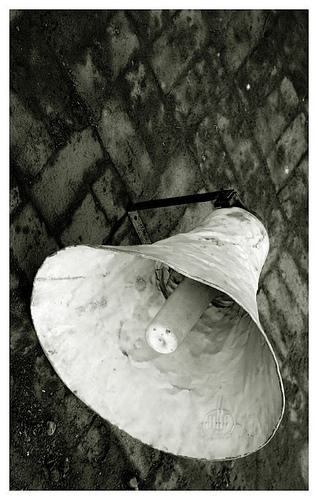
\includegraphics[width=0.115\textwidth]{Images/Comparable/figure1_similarities/original/37729.jpeg}&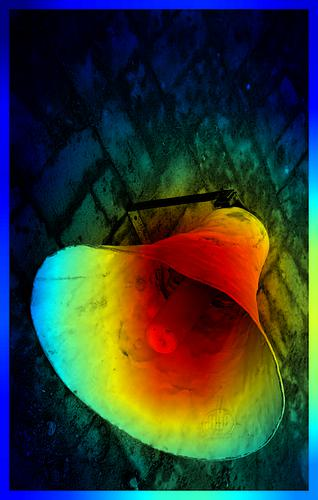
\includegraphics[width=0.115\textwidth]{Images/Comparable/figure1_similarities/raw_att/37729.jpeg}&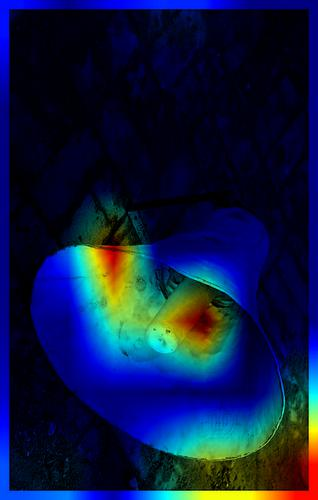
\includegraphics[width=0.115\textwidth]{Images/Comparable/figure1_similarities/shelf_gradcam/37729.jpeg}&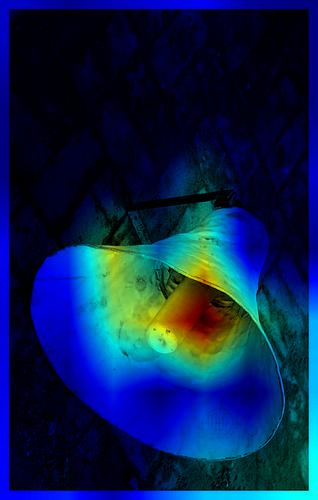
\includegraphics[width=0.115\textwidth]{Images/Comparable/figure1_similarities/gradcam/37729.jpeg}&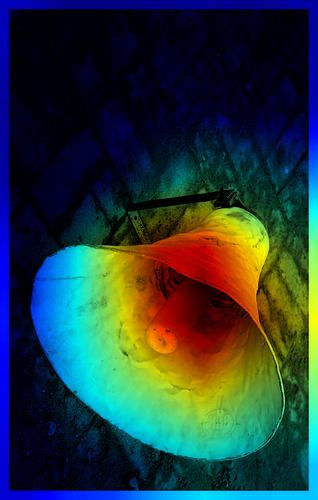
\includegraphics[width=0.115\textwidth]{Images/Comparable/figure1_similarities/shelf_gradcampp/37729.jpeg}&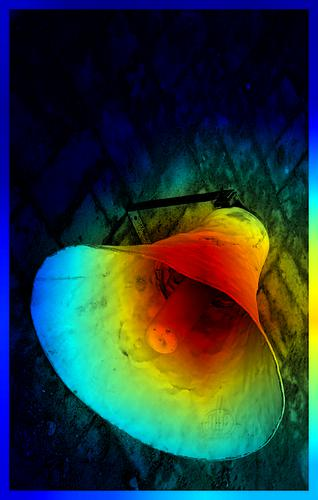
\includegraphics[width=0.115\textwidth]{Images/Comparable/figure1_similarities/gradcampp/37729.jpeg}&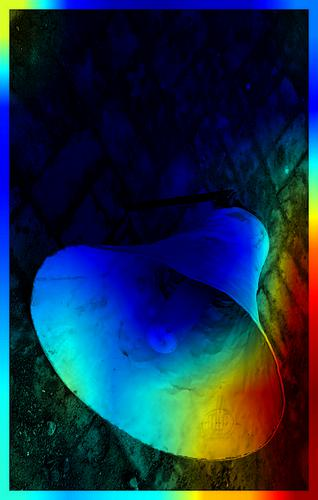
\includegraphics[width=0.115\textwidth]{Images/Comparable/figure1_similarities/scorecam/37729.jpeg}&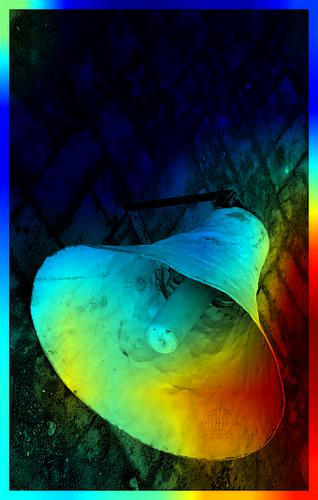
\includegraphics[width=0.115\textwidth]{Images/Comparable/figure1_similarities/shelf_scorecam/37729.jpeg}\\

    {\rotatebox{90}{\tiny Envelope}}&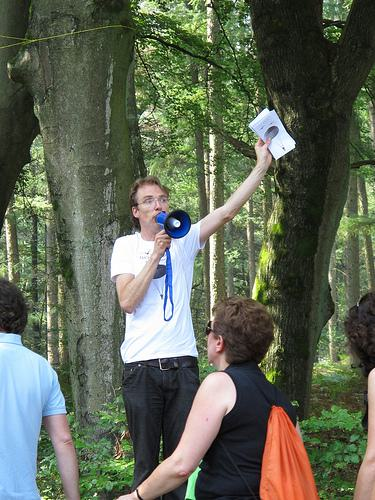
\includegraphics[width=0.115\textwidth]{Images/Comparable/figure1_similarities/original/23541.jpeg}&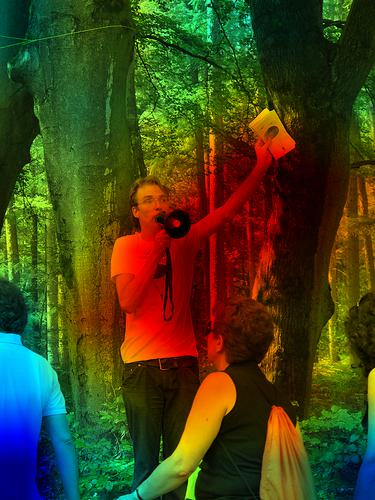
\includegraphics[width=0.115\textwidth]{Images/Comparable/figure1_similarities/raw_att/23541.jpeg}&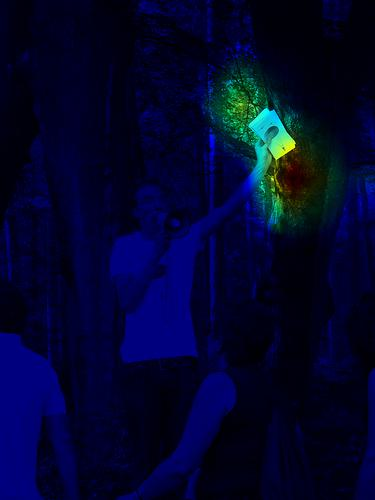
\includegraphics[width=0.115\textwidth]{Images/Comparable/figure1_similarities/shelf_gradcam/23541.jpeg}&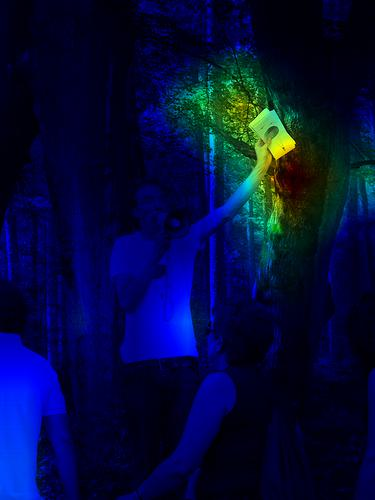
\includegraphics[width=0.115\textwidth]{Images/Comparable/figure1_similarities/gradcam/23541.jpeg}&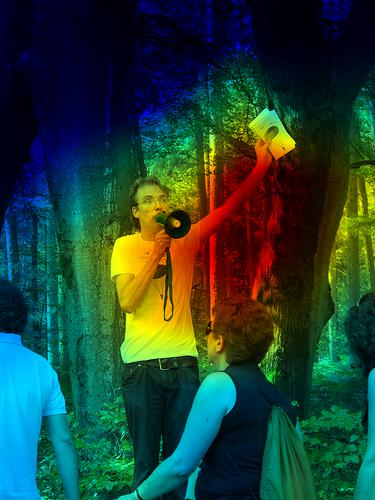
\includegraphics[width=0.115\textwidth]{Images/Comparable/figure1_similarities/shelf_gradcampp/23541.jpeg}&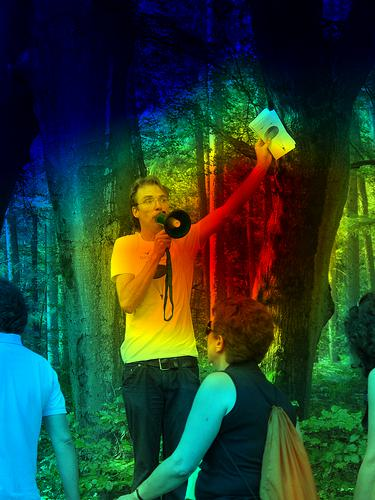
\includegraphics[width=0.115\textwidth]{Images/Comparable/figure1_similarities/gradcampp/23541.jpeg}&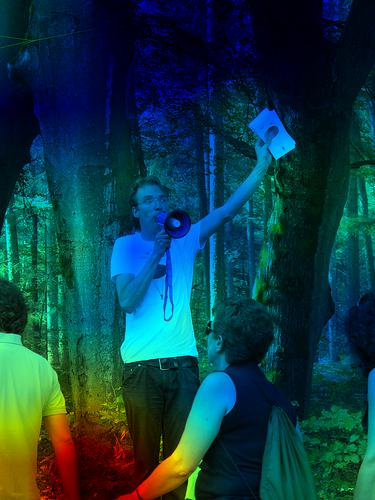
\includegraphics[width=0.115\textwidth]{Images/Comparable/figure1_similarities/scorecam/23541.jpeg}&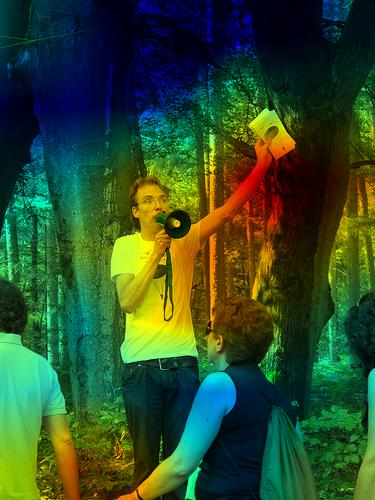
\includegraphics[width=0.115\textwidth]{Images/Comparable/figure1_similarities/shelf_scorecam/23541.jpeg}\\

    {\rotatebox{90}{\tiny Groom}}&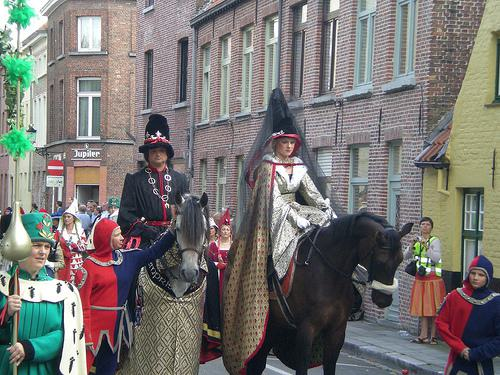
\includegraphics[width=0.115\textwidth]{Images/Comparable/figure1_similarities/original/9602.jpeg}&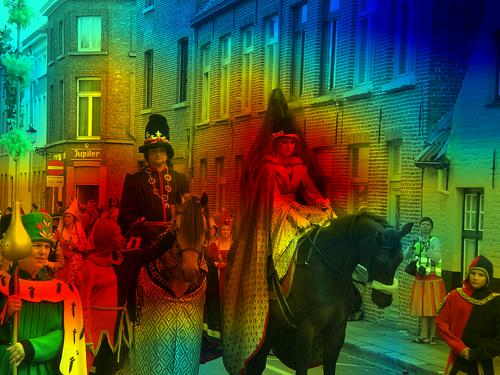
\includegraphics[width=0.115\textwidth]{Images/Comparable/figure1_similarities/raw_att/9602.jpeg}&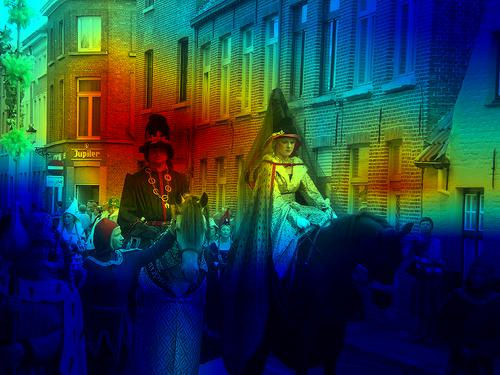
\includegraphics[width=0.115\textwidth]{Images/Comparable/figure1_similarities/shelf_gradcam/9602.jpeg}&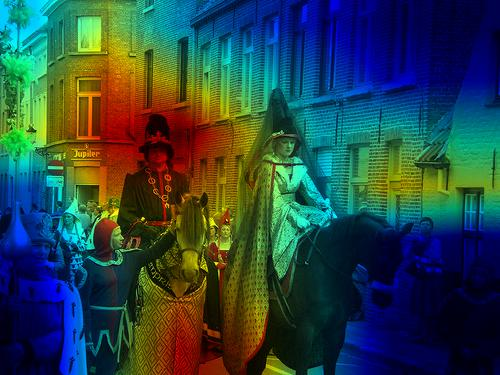
\includegraphics[width=0.115\textwidth]{Images/Comparable/figure1_similarities/gradcam/9602.jpeg}&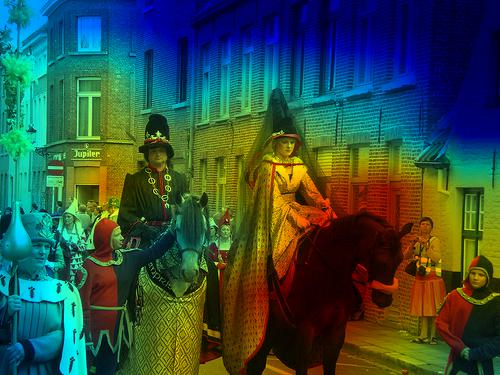
\includegraphics[width=0.115\textwidth]{Images/Comparable/figure1_similarities/shelf_gradcampp/9602.jpeg}&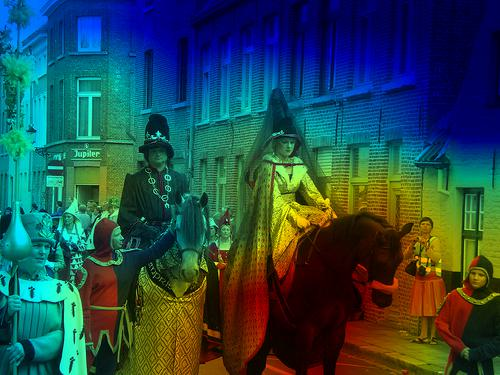
\includegraphics[width=0.115\textwidth]{Images/Comparable/figure1_similarities/gradcampp/9602.jpeg}&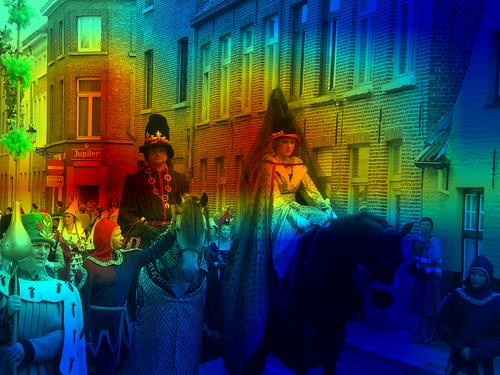
\includegraphics[width=0.115\textwidth]{Images/Comparable/figure1_similarities/scorecam/9602.jpeg}&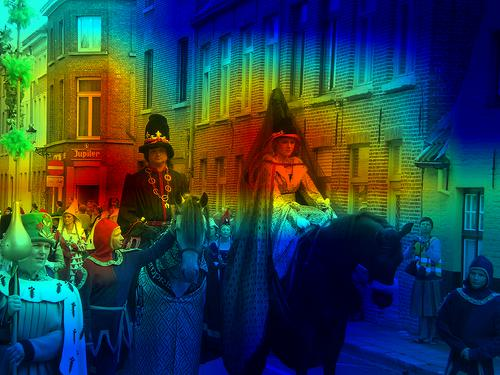
\includegraphics[width=0.115\textwidth]{Images/Comparable/figure1_similarities/shelf_scorecam/9602.jpeg}\\

    {\rotatebox{90}{\tiny Nematode}}&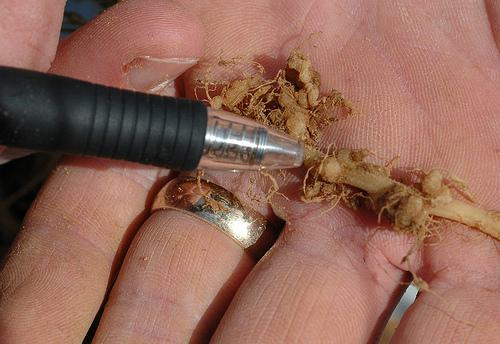
\includegraphics[width=0.115\textwidth]{Images/Comparable/figure1_similarities/original/12414.jpeg}&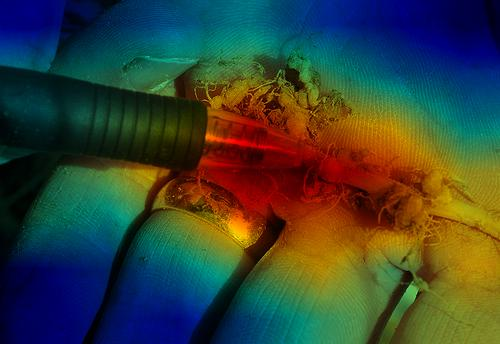
\includegraphics[width=0.115\textwidth]{Images/Comparable/figure1_similarities/raw_att/12414.jpeg}&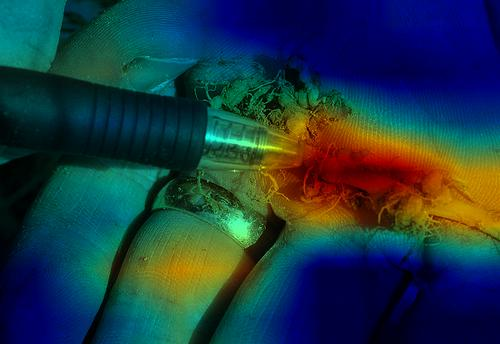
\includegraphics[width=0.115\textwidth]{Images/Comparable/figure1_similarities/shelf_gradcam/12414.jpeg}&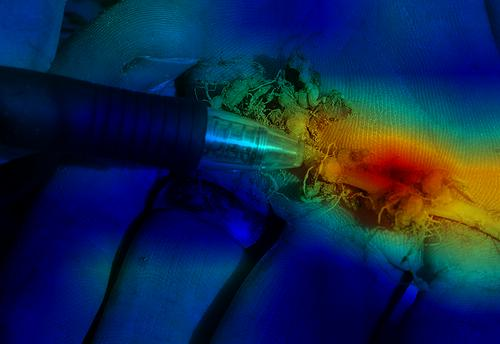
\includegraphics[width=0.115\textwidth]{Images/Comparable/figure1_similarities/gradcam/12414.jpeg}&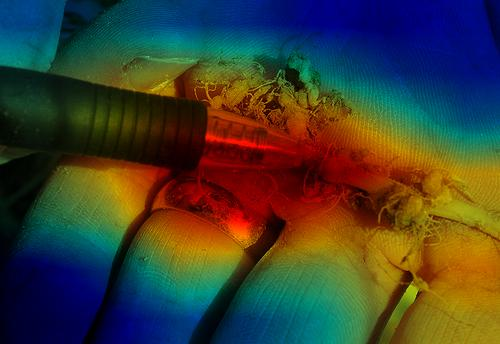
\includegraphics[width=0.115\textwidth]{Images/Comparable/figure1_similarities/shelf_gradcampp/12414.jpeg}&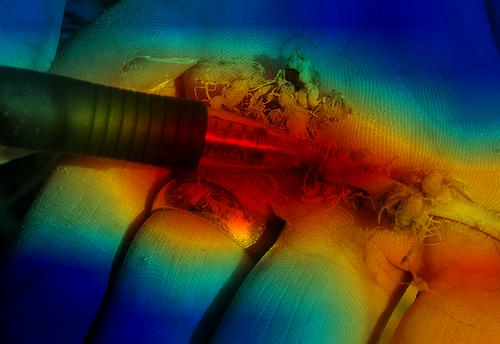
\includegraphics[width=0.115\textwidth]{Images/Comparable/figure1_similarities/gradcampp/12414.jpeg}&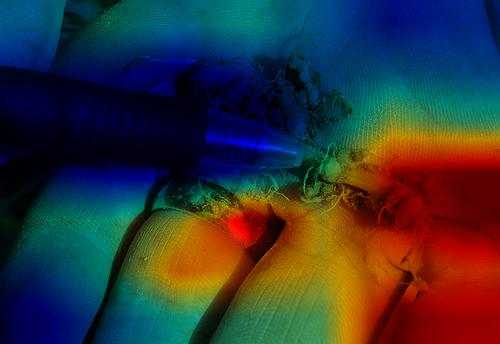
\includegraphics[width=0.115\textwidth]{Images/Comparable/figure1_similarities/scorecam/12414.jpeg}&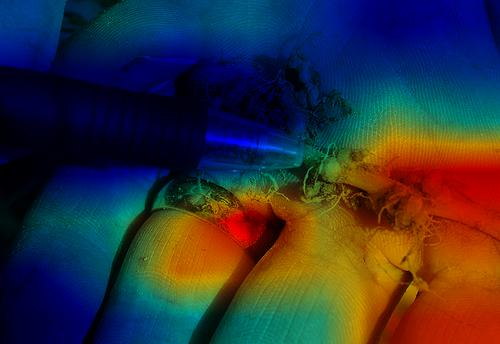
\includegraphics[width=0.115\textwidth]{Images/Comparable/figure1_similarities/shelf_scorecam/12414.jpeg}\\

	% {\rotatebox{90}{\tiny Waffle Iron}}&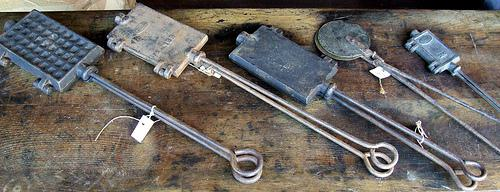
\includegraphics[width=0.115\textwidth]{Images/Comparable/figure1_revisit/original/15749.jpeg}&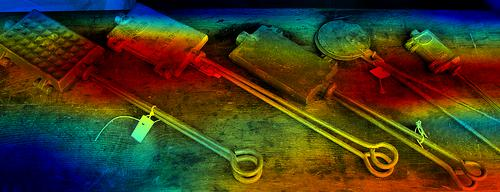
\includegraphics[width=0.115\textwidth]{Images/Comparable/figure1_revisit/raw_att/15749.jpeg}&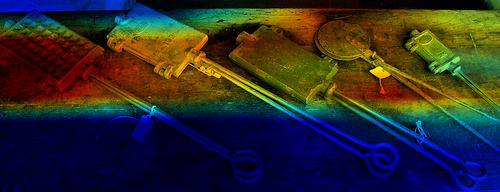
\includegraphics[width=0.115\textwidth]{Images/Comparable/figure1_revisit/shelf_gradcam/15749.jpeg}&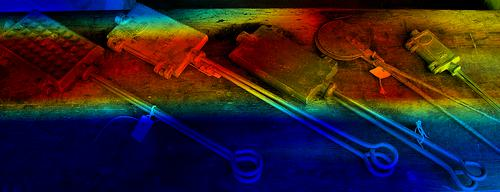
\includegraphics[width=0.115\textwidth]{Images/Comparable/figure1_revisit/gradcam/15749.jpeg}&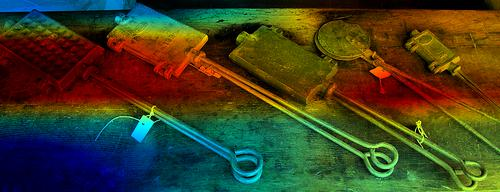
\includegraphics[width=0.115\textwidth]{Images/Comparable/figure1_revisit/shelf_gradcampp/15749.jpeg}&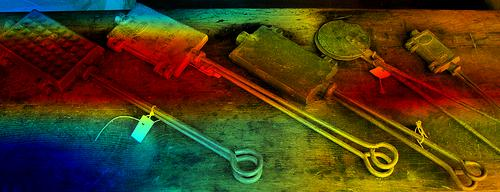
\includegraphics[width=0.115\textwidth]{Images/Comparable/figure1_revisit/gradcampp/15749.jpeg}&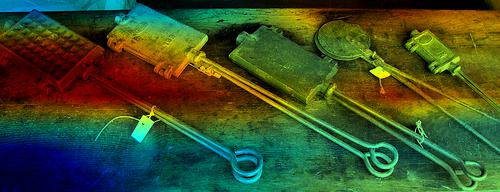
\includegraphics[width=0.115\textwidth]{Images/Comparable/figure1_revisit/scorecam/15749.jpeg}&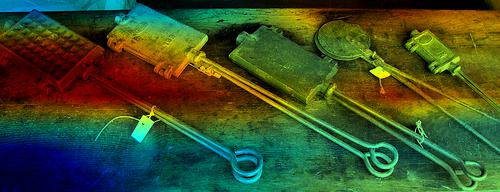
\includegraphics[width=0.115\textwidth]{Images/Comparable/figure1_revisit/scorecam/15749.jpeg}\\

	% {\rotatebox{90}{\tiny Wallaby}}&\multicolumn{1}{c}{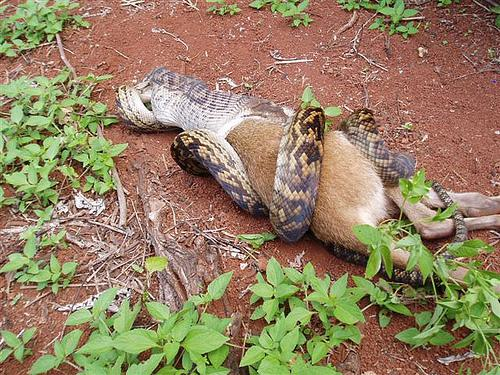
\includegraphics[width=0.115\textwidth]{Images/Comparable/figure1_revisit/original/24263.jpeg}}&\multicolumn{1}{c}{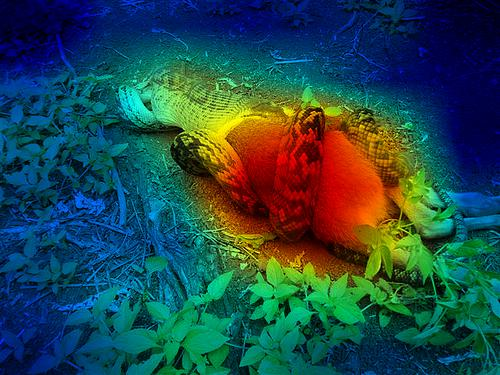
\includegraphics[width=0.115\textwidth]{Images/Comparable/figure1_revisit/raw_att/24263.jpeg}}&\multicolumn{1}{c}{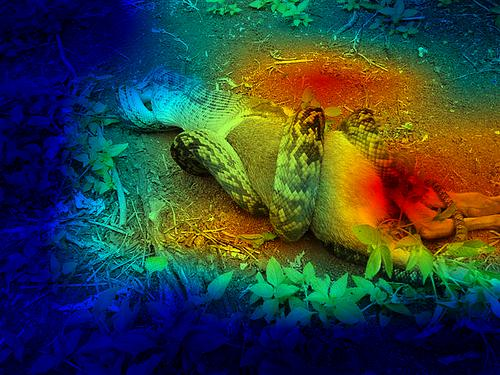
\includegraphics[width=0.115\textwidth]{Images/Comparable/figure1_revisit/shelf_gradcam/24263.jpeg}}&\multicolumn{1}{c}{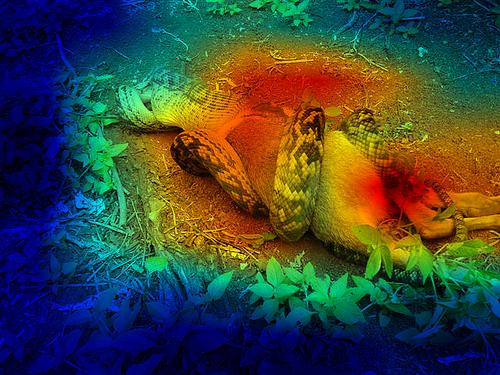
\includegraphics[width=0.115\textwidth]{Images/Comparable/figure1_revisit/gradcam/24263.jpeg}}&\multicolumn{1}{c}{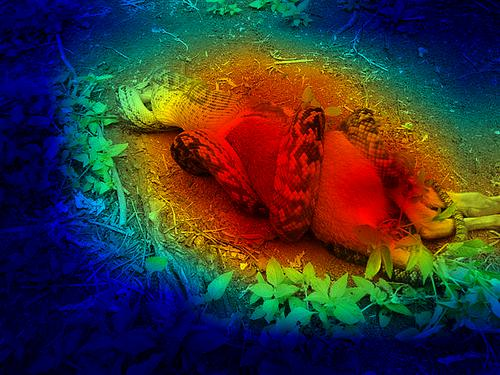
\includegraphics[width=0.115\textwidth]{Images/Comparable/figure1_revisit/shelf_gradcampp/24263.jpeg}}&\multicolumn{1}{c}{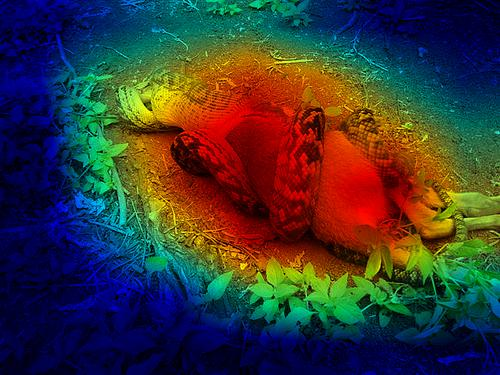
\includegraphics[width=0.115\textwidth]{Images/Comparable/figure1_revisit/gradcampp/24263.jpeg}}&\multicolumn{1}{c}{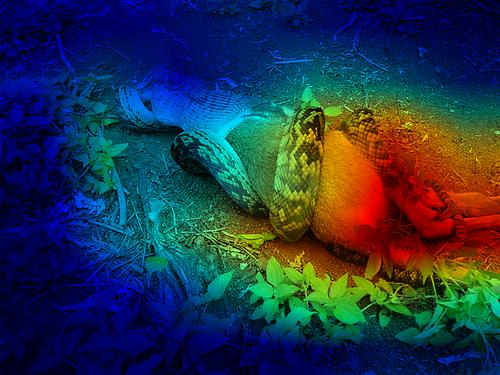
\includegraphics[width=0.115\textwidth]{Images/Comparable/figure1_revisit/scorecam/24263.jpeg}}&\multicolumn{1}{c}{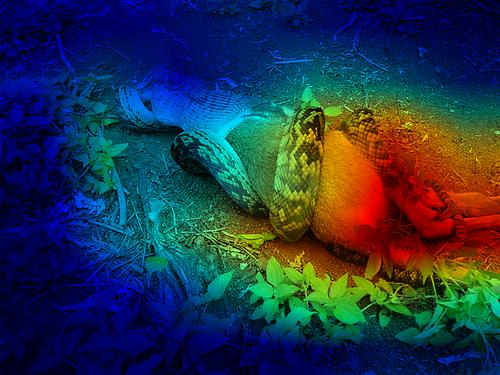
\includegraphics[width=0.115\textwidth]{Images/Comparable/figure1_revisit/scorecam/24263.jpeg}}\\

	% {\rotatebox{90}{\tiny Hoopskirt}}&\multicolumn{1}{c}{\includegraphics[width=0.115\textwidth]{Images/Comparable/figure1_revisit/original/33003.jpeg}}&\multicolumn{1}{c}{\includegraphics[width=0.115\textwidth]{Images/Comparable/figure1_revisit/raw_att/33003.jpeg}}&\multicolumn{1}{c}{\includegraphics[width=0.115\textwidth]{Images/Comparable/figure1_revisit/shelf_gradcam/33003.jpeg}}&\multicolumn{1}{c}{\includegraphics[width=0.115\textwidth]{Images/Comparable/figure1_revisit/gradcam/33003.jpeg}}&\multicolumn{1}{c}{\includegraphics[width=0.115\textwidth]{Images/Comparable/figure1_revisit/shelf_gradcampp/33003.jpeg}}&\multicolumn{1}{c}{\includegraphics[width=0.115\textwidth]{Images/Comparable/figure1_revisit/gradcampp/33003.jpeg}}&\multicolumn{1}{c}{\includegraphics[width=0.115\textwidth]{Images/Comparable/figure1_revisit/scorecam/33003.jpeg}}&\multicolumn{1}{c}{\includegraphics[width=0.115\textwidth]{Images/Comparable/figure1_revisit/scorecam/33003.jpeg}}\\

	% {\rotatebox{90}{\tiny Matchstick}}&\multicolumn{1}{c}{\includegraphics[width=0.115\textwidth]{Images/Comparable/figure1_revisit/original/48096.jpeg}}&\multicolumn{1}{c}{\includegraphics[width=0.115\textwidth]{Images/Comparable/figure1_revisit/raw_att/48096.jpeg}}&\multicolumn{1}{c}{\includegraphics[width=0.115\textwidth]{Images/Comparable/figure1_revisit/shelf_gradcam/48096.jpeg}}&\multicolumn{1}{c}{\includegraphics[width=0.115\textwidth]{Images/Comparable/figure1_revisit/gradcam/48096.jpeg}}&\multicolumn{1}{c}{\includegraphics[width=0.115\textwidth]{Images/Comparable/figure1_revisit/shelf_gradcampp/48096.jpeg}}&\multicolumn{1}{c}{\includegraphics[width=0.115\textwidth]{Images/Comparable/figure1_revisit/gradcampp/48096.jpeg}}&\multicolumn{1}{c}{\includegraphics[width=0.115\textwidth]{Images/Comparable/figure1_revisit/scorecam/48096.jpeg}}&\multicolumn{1}{c}{\includegraphics[width=0.115\textwidth]{Images/Comparable/figure1_revisit/scorecam/48096.jpeg}}\\

	% {\rotatebox{90}{\tiny Sweatshirt}}&\multicolumn{1}{c}{\includegraphics[width=0.115\textwidth]{Images/Comparable/figure1/original/18939.jpeg}}&\multicolumn{1}{c}{\includegraphics[width=0.115\textwidth]{Images/Comparable/figure1/raw_att/18939.jpeg}}&\multicolumn{1}{c}{\includegraphics[width=0.115\textwidth]{Images/Comparable/figure1/shelf_gradcam/18939.jpeg}}&\multicolumn{1}{c}{\includegraphics[width=0.115\textwidth]{Images/Comparable/figure1/gradcam/18939.jpeg}}&\multicolumn{1}{c}{\includegraphics[width=0.115\textwidth]{Images/Comparable/figure1/shelf_gradcampp/18939.jpeg}}&\multicolumn{1}{c}{\includegraphics[width=0.115\textwidth]{Images/Comparable/figure1/gradcampp/18939.jpeg}}&\multicolumn{1}{c}{\includegraphics[width=0.115\textwidth]{Images/Comparable/figure1/shelf_scorecam/18939.jpeg}}&\multicolumn{1}{c}{\includegraphics[width=0.115\textwidth]{Images/Comparable/figure1/scorecam/18939.jpeg}}\\

	{\rotatebox{90}{\tiny CRT screen}}&\multicolumn{1}{c}{\includegraphics[width=0.115\textwidth]{Images/Comparable/figure1/original/43057.jpeg}}&\multicolumn{1}{c}{\includegraphics[width=0.115\textwidth]{Images/Comparable/figure1/raw_att/43057.jpeg}}&\multicolumn{1}{c}{\includegraphics[width=0.115\textwidth]{Images/Comparable/figure1/shelf_gradcam/43057.jpeg}}&\multicolumn{1}{c}{\includegraphics[width=0.115\textwidth]{Images/Comparable/figure1/gradcam/43057.jpeg}}&\multicolumn{1}{c}{\includegraphics[width=0.115\textwidth]{Images/Comparable/figure1/shelf_gradcampp/43057.jpeg}}&\multicolumn{1}{c}{\includegraphics[width=0.115\textwidth]{Images/Comparable/figure1/gradcampp/43057.jpeg}}&\multicolumn{1}{c}{\includegraphics[width=0.115\textwidth]{Images/Comparable/figure1/shelf_scorecam/43057.jpeg}}&\multicolumn{1}{c}{\includegraphics[width=0.115\textwidth]{Images/Comparable/figure1/scorecam/43057.jpeg}}\\ % Checked 

   {\rotatebox{90}{\tiny Snowboard}}&\includegraphics[width=0.115\textwidth]{Images/Comparable/figure1_similarities/original/11376.jpeg}&\includegraphics[width=0.115\textwidth]{Images/Comparable/figure1_similarities/raw_att/11376.jpeg}&\includegraphics[width=0.115\textwidth]{Images/Comparable/figure1_similarities/shelf_gradcam/11376.jpeg}&\includegraphics[width=0.115\textwidth]{Images/Comparable/figure1_similarities/gradcam/11376.jpeg}&\includegraphics[width=0.115\textwidth]{Images/Comparable/figure1_similarities/shelf_gradcampp/11376.jpeg}&\includegraphics[width=0.115\textwidth]{Images/Comparable/figure1_similarities/gradcampp/11376.jpeg}&\includegraphics[width=0.115\textwidth]{Images/Comparable/figure1_similarities/scorecam/11376.jpeg}&\includegraphics[width=0.115\textwidth]{Images/Comparable/figure1_similarities/shelf_scorecam/11376.jpeg}\\

 
\end{tabular}
% }
\vspace{3pt}
\caption{Comparison of saliency maps generated by different CAM-based methods, using GAP and our \Ours, on ImageNet images. The raw attention is the one used for pooling by \Ours.}
\label{fig:compmethods}
\end{figure*}
%------------------------------------------------------------------------------

%------------------------------------------------------------------------------

\subsection{Qualitative evaluation}
\label{subsec:vinspection}

We show saliency maps obtained by different interpretability methods using either \gap or \Ours, as well as the class-agnostic raw attention coming from our \Ours, see \autoref{fig:compmethods}.
%, including the class-agnostic raw attention obtained by \Ours.

We observe that the raw attention focuses on objects of interest in the images. 
%\textcolor{orange}{
In general, saliency maps obtained with \Ours are similar but tend to cover larger regions of the object or more instances compared with \gap.%, see \autoref{fig:compmethods}.
%, for example in the ``CRT screen'' image in \autoref{fig:compmethods}. 
%}
%
Indeed, the differences in saliency maps should not be large, as both methods share the same features maps $F^k_\ell$ and only the weight coefficients $\alpha^c_k$ differ.
Despite the small differences, the following quantitative results show that \Ours has a significant impact on the interpretability metrics.

%
%\textcolor{red}{
%As a further investigation, we compute cosine similarities of saliency maps and obtain 0.998 (or 6.49\% euclidean distance), averaged over the dataset. We then observed a similarity of 0.752 for the pooled features and 0.612 for the gradient.
%Finally, the percentage difference in probability for the ground truth class is of 27.8\% on average.
%These results show that the small changes in the saliency maps are meaningful.
%}


%In some examples, the saliency maps obtained are quite similar.%using \gap and \Ours are not very different. 
%The differences are expected to be low, as both methods share the same features maps $F^k_\ell$ and only the weight coefficients $\alpha^c_k$ differ.
%%, while the CAM-based methods have their own mechanism to focus on what is relevant for the prediction of the class of interest. 
%Despite the small visual differences, the following quantitative results show that \Ours has a significant impact on the interpretability metrics.

%------------------------------------------------------------------------------
\begin{figure}[t]
\scriptsize
\centering
\setlength{\tabcolsep}{1.3pt}
%    \resizebox{\columnwidth}{!}{%
     \begin{tabular}{cccccccc}
           \mc{2}{Corridor}&\mc{2}{Greenhouse}&\mc{2}{Pool Inside}&\mc{2}{Wine Cellar}\\
           Input image&Raw Attention&Input image&Raw Attention&Input image&Raw Attention&Input image&Raw Attention\\
           \includegraphics[width=0.12\textwidth,height=0.08\textwidth]{fig/castream/images/Outdataset/Corridor/Original/c1.jpg}&
           \includegraphics[width=0.12\textwidth,height=0.08\textwidth]{fig/castream/images/Outdataset/Corridor/Attention/c1.jpg}&
           \includegraphics[width=0.12\textwidth,height=0.08\textwidth]{fig/castream/images/Outdataset/Greenhouse/Original/celosie_02.jpg}&
           \includegraphics[width=0.12\textwidth,height=0.08\textwidth]{fig/castream/images/Outdataset/Greenhouse/Attention/celosie_02.jpg}&
           \includegraphics[width=0.12\textwidth,height=0.08\textwidth]{fig/castream/images/Outdataset/Poolinside/Original/003_1b.jpg}&
           \includegraphics[width=0.12\textwidth,height=0.08\textwidth]{fig/castream/images/Outdataset/Poolinside/Attention/003_1b.jpg}&
           \includegraphics[width=0.12\textwidth,height=0.08\textwidth]{fig/castream/images/Outdataset/WineCellar/Original/bodega2.jpg}&
           \includegraphics[width=0.12\textwidth,height=0.08\textwidth]{fig/castream/images/Outdataset/WineCellar/Attention/bodega2.jpg}\\
           
           \includegraphics[width=0.12\textwidth,height=0.08\textwidth]{fig/castream/images/Outdataset/Corridor/Original/1L_10_Corridor_A.jpg}&
           \includegraphics[width=0.12\textwidth,height=0.08\textwidth]{fig/castream/images/Outdataset/Corridor/Attention/1L_10_Corridor_A.jpg}&
           \includegraphics[width=0.12\textwidth,height=0.08\textwidth]{fig/castream/images/Outdataset/Greenhouse/Original/20070417klpcnatun_229_Ies_SCO.jpg}&
           \includegraphics[width=0.12\textwidth,height=0.08\textwidth]{fig/castream/images/Outdataset/Greenhouse/Attention/20070417klpcnatun_229_Ies_SCO.jpg}&
           \includegraphics[width=0.12\textwidth,height=0.08\textwidth]{fig/castream/images/Outdataset/Poolinside/Original/141821195_M.jpg}&
           \includegraphics[width=0.12\textwidth,height=0.08\textwidth]{fig/castream/images/Outdataset/Poolinside/Attention/141821195_M.jpg}&
           \includegraphics[width=0.12\textwidth,height=0.08\textwidth]{fig/castream/images/Outdataset/WineCellar/Original/bodega_45_18_yahoo.jpg}&
           \includegraphics[width=0.12\textwidth,height=0.08\textwidth]{fig/castream/images/Outdataset/WineCellar/Attention/bodega_45_18_yahoo.jpg}\\
           
           \includegraphics[width=0.12\textwidth,height=0.08\textwidth]{fig/castream/images/Outdataset/Corridor/Original/430_Korridor_300.jpg}&
           \includegraphics[width=0.12\textwidth,height=0.08\textwidth]{fig/castream/images/Outdataset/Corridor/Attention/430_Korridor_300.jpg}&
           \includegraphics[width=0.12\textwidth,height=0.08\textwidth]{fig/castream/images/Outdataset/Greenhouse/Original/20070418klpcnaecl_364_Ies_SCO.jpg}&
           \includegraphics[width=0.12\textwidth,height=0.08\textwidth]{fig/castream/images/Outdataset/Greenhouse/Attention/20070418klpcnaecl_364_Ies_SCO.jpg}&
           \includegraphics[width=0.12\textwidth,height=0.08\textwidth]{fig/castream/images/Outdataset/Poolinside/Original/catalogue_piscine_interieur.jpg}&
           \includegraphics[width=0.12\textwidth,height=0.08\textwidth]{fig/castream/images/Outdataset/Poolinside/Attention/catalogue_piscine_interieur.jpg}&
           \includegraphics[width=0.12\textwidth,height=0.08\textwidth]{fig/castream/images/Outdataset/WineCellar/Original/bodega_63_24_flickr.jpg}&
           \includegraphics[width=0.12\textwidth,height=0.08\textwidth]{fig/castream/images/Outdataset/WineCellar/Attention/bodega_63_24_flickr.jpg}\\
           
           \includegraphics[width=0.12\textwidth,height=0.08\textwidth]{fig/castream/images/Outdataset/Corridor/Original/06_Right_corridor_of_the_main_hall.jpg}&
           \includegraphics[width=0.12\textwidth,height=0.08\textwidth]{fig/castream/images/Outdataset/Corridor/Attention/06_Right_corridor_of_the_main_hall.jpg}&
           \includegraphics[width=0.12\textwidth,height=0.08\textwidth]{fig/castream/images/Outdataset/Greenhouse/Original/2026_2006_Grimm_s_Gardens_Greenhouse.jpg}&
           \includegraphics[width=0.12\textwidth,height=0.08\textwidth]{fig/castream/images/Outdataset/Greenhouse/Attention/2026_2006_Grimm_s_Gardens_Greenhouse.jpg}&
           \includegraphics[width=0.12\textwidth,height=0.08\textwidth]{fig/castream/images/Outdataset/Poolinside/Original/connolly_center_pool_inside_lg.jpg}&
           \includegraphics[width=0.12\textwidth,height=0.08\textwidth]{fig/castream/images/Outdataset/Poolinside/Attention/connolly_center_pool_inside_lg.jpg}&
           \includegraphics[width=0.12\textwidth,height=0.08\textwidth]{fig/castream/images/Outdataset/WineCellar/Original/bodega_78_08_flickr.jpg}&
           \includegraphics[width=0.12\textwidth,height=0.08\textwidth]{fig/castream/images/Outdataset/WineCellar/Attention/bodega_78_08_flickr.jpg}\\              
    \end{tabular}
%    }
    \vspace{3pt}
    \caption{\textbf{Raw attention maps} obtained from our \Ours on images of the MIT 67 Scenes dataset \autocite{quattoni2009recognizing} on classes that do not exist in ImageNet. The network sees them at inference for the first time.} 
    %
    \label{fig:enter-label}
\end{figure}
%------------------------------------------------------------------------------

In addition, \autoref{fig:enter-label} shows examples of images from the MIT 67 Scenes dataset~\cite{quattoni2009recognizing} along with raw attention maps obtained by \Ours. These images come from four classes that do not exist in ImageNet and the network sees them at inference for the first time. Nevertheless, the attention maps focus on objects of interest in general.

\subsection{Interpretabity metrics}
\label{subsec:interecon}

%------------------------------------------------------------------------------
\begin{table}
\centering
\scriptsize
\setlength{\tabcolsep}{3.5pt}
% \resizebox{\columnwidth}{!}{%
\begin{tabular}{llcccccc}\toprule
	\mc{8}{\Th{Accuracy and Parameters}}\\\midrule
	\Th{Network}&\mc{1}{\Th{Pool}}&\Th{GFLOPs}&\mc{2}{\Th{$\#$Param}}&\mc{2}{\Th{Param$\%$}}&\Th{Acc$\uparrow$}\\\midrule
	\mr{2}{\Th{ResNet-18}}&\mc{1}{\gap}&3.648&\mc{2}{11.69M}&\mc{2}{\mr{2}{3.71}}&67.28\\
		&\mc{1}{\ours}&3.652&\mc{2}{12.13M}&&&67.54\\\midrule
	\mr{2}{\Th{ResNet-50}}&\mc{1}{\gap}&8.268&\mc{2}{25.56M}&\mc{2}{\mr{2}{27.27}}&74.55\\
		&\mc{1}{\ours}&8.288&\mc{2}{32.53M}&&&74.70\\\midrule
	\mr{2}{\Th{ConvNeXt-S}}&\mc{1}{\gap}&17.395&\mc{2}{50.22M}&\mc{2}{\mr{2}{1.95}}&83.26\\
		&\mc{1}{\ours}&17.400&\mc{2}{51.20M}&&&83.14\\\midrule
	\mr{2}{\Th{ConvNeXt-B}}&\mc{1}{\gap}&30.747&\mc{2}{88.59M}&\mc{2}{\mr{2}{1.96}}&83.72\\
		&\mc{1}{\ours}&30.753&\mc{2}{90.33M}&&&83.51\\\midrule
%	\mr{2}{\Th{ViT-Base}}&&\cls\footnotemark{}&\mc{2}{86.58M}&\mc{2}{\mr{2}{8.18}}&80.01\\
%		&&\ours&\mc{2}{93.66M}&&&74.73\\\midrule
		
	\mc{8}{\Th{Interpretability Metrics}}\\\midrule
	\Th{Network}&\Th{Method}&\Th{Pool}&\Th{AD$\downarrow$}&\Th{AG$\uparrow$}&\Th{AI$\uparrow$}&\Th{I$\uparrow$}&\Th{D$\downarrow$}\\\midrule

	\mr{7}{\Th{ResNet-18}}&\mr{2}{Grad-CAM}&\gap&17.64&12.73&41.21&63.13&\textbf{10.66}\\ %
		& &\ours&\textbf{16.99}&\textbf{17.22}&\textbf{44.95}&\textbf{65.94}&10.68\\\cmidrule{2-8} %
		& \mr{2}{Grad-CAM++}&\gap&19.05&11.16&37.99&62.80&\textbf{10.75}\\ %
		& &\ours&\textbf{19.02}&\textbf{14.76}&\textbf{40.82}&\textbf{65.53}&10.82\\\cmidrule{2-8} %
		& \mr{2}{Score-CAM}&\gap&13.64&12.98&44.53&62.56&\textbf{11.37}\\ %
		& &\ours&\textbf{11.53}&\textbf{18.12}&\textbf{50.32}&\textbf{65.33}&11.51\\\midrule %

	\mr{7}{\Th{ResNet-50}}&\mr{2}{Grad-CAM}&\gap&13.04&17.56&44.47&72.57&\textbf{13.24}\\ %
		& &\ours&\textbf{12.54}&\textbf{22.67}&\textbf{48.56}&\textbf{75.53}&13.50\\\cmidrule{2-8} %
		& \mr{2}{Grad-CAM++}&\gap&\textbf{13.79}&15.87&42.08&72.32&\textbf{13.33}\\ %
		& &\ours&13.99&\textbf{19.29}&\textbf{44.60}&\textbf{75.21}&13.78\\\cmidrule{2-8} %
		& \mr{2}{Score-CAM}&\gap&8.83&17.97&48.46&71.99&\textbf{14.31}\\ %
		& &\ours&\textbf{7.09}&\textbf{23.65}&\textbf{54.20}&\textbf{74.91}&14.68\\\midrule%

	% \multirow{6}{*}{MobileNet-V2}&\mc{2}{Grad-CAM}&\gap&16.11&12.89&40.27&64.47&\textbf{11.92}\\
	%   & &\ours&\textbf{15.53}&\textbf{16.13}&\textbf{42.95}&\textbf{67.80}&12.24\\\cmidrule{2-8}
	%   & \mc{2}{Grad-CAM++}&\gap&17.65&11.12&37.30&64.08&\textbf{11.96}\\
	%   & &\ours&\textbf{17.55}&\textbf{13.52}&\textbf{38.61}&\textbf{67.36}&12.28\\\cmidrule{2-8}
	%   & \mc{2}{Score-CAM}&\gap&12.32&13.52&43.94&64.13&\textbf{12.23}\\
	%   & &\ours&\textbf{10.71}&\textbf{17.35}&\textbf{47.81}&\textbf{67.41}&12.65\\\midrule

	% \multirow{6}{*}{ConvNext Tiny}&\mc{2}{Grad-CAM}&\gap&43.15&2.82&16.58&49.15&\textbf{23.68}\\ % Numbers match, check saliency
	%   & &\ours&\textbf{22.49}&\textbf{14.03}&\textbf{30.65}&\textbf{82.55}&35.22\\\cmidrule{2-8} % Revision running
	%   & \mc{2}{Grad-CAM++}&\gap&43.96&2.45&15.67&48.95&\textbf{23.90}\\ % Pending
	%   & &\ours&\textbf{25.90}&\textbf{12.16}&\textbf{27.70}&\textbf{82.01}&40.42\\\cline{2-8} % Revision running
	%   & \mc{2}{Score-CAM}&\gap&48.25&1.86&13.47&47.12&\textbf{35.38}\\ % Pending
	%   & &\ours&\textbf{19.69}&\textbf{12.42}&\textbf{28.92}&\textbf{80.21}&49.25\\\midrule % Revision running

	\mr{7}{\Th{ConvNeXt-S}}&\mr{2}{Grad-CAM}&\gap&42.99&1.69&12.60&48.42&\textbf{30.12}\\ % Numbers match, check saliency
		& &\ours&\textbf{22.09}&\textbf{14.91}&\textbf{32.65}&\textbf{84.82}&43.02\\\cmidrule{2-8} % Revision running
		& \mr{2}{Grad-CAM++}&\gap&56.42&1.32&10.35&48.28&\textbf{33.41}\\ % Pending
		& &\ours&\textbf{51.87}&\textbf{9.40}&\textbf{20.55}&\textbf{84.28}&52.58\\\cmidrule{2-8} % Revision running
		& \mr{2}{Score-CAM}&\gap&74.79&1.29&10.10&47.40&\textbf{38.21}\\ % Pending
		& &\ours&\textbf{64.21}&\textbf{8.81}&\textbf{18.96}&\textbf{82.92}&57.46\\\midrule % Revision running

	\mr{7}{\Th{ConvNeXt-B}}&\mr{2}{Grad-CAM}&\gap&33.72&2.43&15.25&52.85&\textbf{29.57}\\ % Pending
		& &\ours&\textbf{19.45}&\textbf{13.96}&\textbf{32.89}&\textbf{86.38}&45.29\\\cmidrule{2-8} % Revision running
		& \mr{2}{Grad-CAM++}&\gap&\textbf{34.01}&2.37&15.60&52.83&\textbf{29.17}\\ % Pending
		& &\ours&36.69&\textbf{8.00}&\textbf{21.95}&\textbf{85.39}&53.42\\\cmidrule{2-8} % Revision running
		& \mr{2}{Score-CAM}&\gap&43.55&2.23&15.67&50.96&\textbf{39.49}\\ % Pending
		& &\ours&\textbf{23.51}&\textbf{11.04}&\textbf{27.35}&\textbf{83.41}&60.53\\\midrule% Revision running

%	\mr{7}{\Th{ViT-B}}&\mr{2}{Grad-CAM}&\cls\footnotemark[\value{footnote}]&83.66&1.49&7.37&66.43&34.98\\ % Pending
%		& &\ours&49.88&4.07&16.10&67.12&10.25\\\cmidrule{2-8} % Revision running
%		& \mr{2}{Grad-CAM++}&\cls\footnotemark[\value{footnote}]&97.03&0.01&1.36&\textbf{66.80}&33.35\\ % Pending
%		& &\ours&74.81&1.64&7.43&61.95&28.29\\\cmidrule{2-8} % Revision running
%		& \mr{2}{Score-CAM}&\cls\footnotemark[\value{footnote}]&TBA&TBA&TBA&TBA&TBA\\ % Pending
%		& &\ours&TBA&TBA&TBA&TBA&TBA\\\bottomrule % Revision running
\end{tabular}
% }
%\vspace{3pt}
\caption{\emph{Accuracy, parameters and interpretability metrics} of \Ours \vs baseline \gap for different networks and interpretability methods on ImageNet. \Th{$\#$Param}: total parameters; \Th{Param$\%$}: percentage of \Ours parameters relative to backbone.}
\label{tab:intrecon-all}
\end{table}
%------------------------------------------------------------------------------
% \footnotetext{Built-in \cls token from Vision Transformers.}    
%------------------------------------------------------------------------------

Here we measure the effect of employing our \Ours approach to pool features \vs the baseline \gap on the faithfulness of explanations, using classification metrics for interpretability. Results are reported in \autoref{tab:intrecon-all} for ImageNet and  \autoref{tab:pascal} for CUB and Pascal VOC.

\autoref{tab:intrecon-all} shows that for different networks, CAM-based interpretability methods and dataset, \Ours provides consistent improvements over \gap in terms of AD, AG, AI and I metrics, while performing lower on D. 
%
%\textcolor{red}{
Deletion has raised concerns in previous works \cite{chefer2021transformer, zhang2023opti}. Indeed, it gradually replaces pixels by black, unlike insertion which starts from a blurred image. This poses the problem of \emph{out-of-distribution} (OOD) data~\cite{gomez2022metrics, hase2021outofdistribution, qiu2021resisting}, possibly introducing bias related to the shape of black regions~\cite{rong2022consistent}. Moreover, non-spread saliency maps tend to perform better \cite{zhang2023opti}, which is likely the reason for lower performance. %We suppose that erasing one main object area is more efficient.  
%}

%\textcolor{orange}{Considering that saliency maps of the two pooling methods do not present large differences, the observed improvement in interpretability metrics can be attributed to the predictive power of the learned attention mechanism. 
%}

%That is, class probabilities can change due to attention, even if saliency maps, obtained features and predictions are the same.}
%\textcolor{red}{
Results on CUB in \autoref{tab:pascal} show that our \Ours consistently provides improvements when the model is finetuned on a smaller fine-grained dataset.
%}

%Table \autoref{tab:pascal} present interpretability results for the PASCAL dataset \cite{Everingham15}.
% \textcolor{red}{
Regarding Pascal VOC, the results for Score-CAM are similar to the ones on ImageNet and CUB, with consistent improvements on all metrics but Deletion. 
However, Grad-CAM and Grad-CAM++ only provide improvements on Average Gain and Average Increase. Average Drop, Insertion and Deletion are very similar.
In fact, Pascal VOC is a multi-class dataset and  our \Ours is class agnostic. Thus, the attention-based pooling is the same for different class for a given image, which reduces the benefit of our \Ours.
%We believe the fact that 
% }

It is also interesting to observe the performance of Score-CAM, as it computes channel weights $\alpha_k^c$ in~\eq{sal} without using gradients. 
In gradient-based methods, channel weights are modified by \Ours due to modified backward gradient flow to features through cross attention blocks rather than \gap.
In Score-CAM however, channel weights are only modified in the forward class probabilities computation, due to attention.

% Regarding the results on ViT-Base, we observe the previously reported failure of CAM based methods on vision transformers\cite{zhang2023opti,chefer2021transformer}; in contrast we note that with the addition of our stream, the interpretability properties \textbf{changes.}

%------------------------------------------------------------------------------

% \subsection{Localization Evaluation}
% \label{subsec:loceval}
% 
% In this section, we assess the localization properties of the saliency maps provided by the inclusion of the CLS stream-based representation. We report these results in table \ref{tab:localization}. It shows that all the localization metrics provide similar scores on different methods and networks. CLS helps saliency maps keep localization information while gaining more classification information. 
% \begin{table}[H]
% 	\centering
% 	%\resizebox{\columnwidth}{!}{%
% 	\scriptsize
% 	\setlength{\tabcolsep}{2pt}
% 	\begin{tabular}{lllccc|cccc}\toprule
% 		\Th{Backbone}&\Th{Method}&\Th{Repr}&\Th{OM$\downarrow$}&\Th{LE$\downarrow$}&\Th{F1$\uparrow$}&\Th{BA$\uparrow$}&\Th{SP$\uparrow$}&\Th{EP$\uparrow$}&\Th{SM$\downarrow$}\\\midrule
% 		\mr{6}{\Th{ResNet-18}}&\mr{2}{\Th{Grad-CAM}}&GAP&\tb{80.6}&61.4&49.1&\tb{58.3}&13.7&13.1&\tb{2.93}\\
% 			& &CLS&81.1&\tb{61.3}&49.1&58.2&13.7&13.1&3.10\\ \cmidrule{3-10}
% 			&\mr{2}{\Th{Grad-CAM++}}&GAP&\tb{80.5}&60.9&50.0&\tb{58.3}&13.7&13.1&\tb{2.89}\\
% 			& &CLS&81.0&60.9&\tb{50.1}&58.0&13.7&13.1&3.07\\\cmidrule{3-10}
% 			&\mr{2}{\Th{Score-CAM}}&GAP&\tb{80.5}&60.9&\tb{49.7}&57.7&13.7&13.1&\tb{2.89}\\
% 			& &CLS&81.0&60.9&49.5&57.3&13.7&13.1&3.07\\ \midrule
% 			\mr{6}{\Th{ResNet-50}}&\mr{2}{\Th{Grad-CAM}}&GAP&80.0&66.4&49.5&58.8&13.8&13.2&\tb{2.56}\\
% 			& &CLS&80.0&66.4&\tb{49.6}&58.8&13.8&13.2&2.62\\\cmidrule{3-10}
% 			&\mr{2}{\Th{Grad-CAM++}}&GAP&\tb{80.2}&\tb{66.7}&50.4&\tb{58.7}&13.9&13.3&\tb{2.55}\\
% 			& &CLS&80.3&66.9&\tb{50.6}&58.0&13.9&13.3&2.64\\\cmidrule{3-10}
% 			&\mr{2}{\Th{Score-CAM}}&GAP&\tb{80.0}&66.3&\tb{50.3}&\tb{57.9}&13.8&13.2&\tb{2.55}\\
% 			& &CLS&80.1&66.3&50.0&57.5&13.8&13.2&2.62\\\bottomrule
% 	\end{tabular}
% 	%}
% 	\caption{Comparison of interpretable localization for ResNet on ImageNet.}
% 	\label{tab:localization}
% \end{table}

%------------------------------------------------------------------------------

\subsection{Classification accuracy}
\label{subsec:classification}

%Here we measure the effect of employing our \Ours approach to pool features \vs the baseline \gap on 

Classification accuracy, number of parameters and GFLOPs for both our \Ours and the baselines are reported in \autoref{tab:intrecon-all} (top part).

By adding our \Ours to the network, classification remains on par with the baseline. Importantly, the network including the classifier remains frozen and the features used for the global image representation remain fixed, meaning that any change in accuracy is due to the attention-based pooling mechanism. 
%
% \textcolor{red}{
We further report the number of GFLOPs for one forward pass and the parameters count of both methods.
Our \Ours has little computation cost and the parameter overhead depends on the embedding dimension because of projection $W_\ell$ in~\eq{qk-layer} and is small in general, except for ResNet-50. Thus, with small overhead in resources, \Ours achieves superior explanations of the classifier predictions, while maintaining accuracy.
% }

%------------------------------------------------------------------------------
\begin{table}
\centering
\scriptsize
\setlength{\tabcolsep}{4pt}
%\resizebox{\columnwidth}{!}{%
\begin{tabular}{llccccc}\toprule                    
	\mc{7}{\textbf{\Th{CUB-200-2011 - ResNet-50}}}\\\midrule
	&\Th{Pooling}&\mc{2}{}&\mc{2}{}&\Th{Acc$\uparrow$}\\\midrule
		&\gap&\mc{2}{}&\mc{2}{}&76.96\\
		&\ours&\mc{2}{}&\mc{2}{}&75.90\\\midrule
	
	\mc{7}{\Th{Interpretability Metrics}}\\\midrule
	\Th{Method}&\Th{Pooling}&AD$\downarrow$&AG$\uparrow$&AI$\uparrow$&I$\uparrow$&D$\downarrow$\\\midrule
	% \multirow{3}{*}{GAP}&\multirow{3}{*}{74.55}&Grad-CAM&13.04&17.56&44.47&72.57&13.24\\
	%  & &Grad-CAM++&13.79&15.87&42.08&72.32&13.33\\
	%  & &Score-CAM&13.64&12.98&44.53&62.56&11.37\\\hline %
	\mr{2}{Grad-CAM}&\gap&10.87&10.29&45.81&65.71&\textbf{6.17}\\
		&\ours&\textbf{10.44}&\textbf{17.61}&\textbf{53.54}&\textbf{74.60}&6.56\\\midrule
	\mr{2}{Grad-CAM++}&\gap&11.35&9.68&44.32&65.64&\textbf{5.92}\\
		&\ours&\textbf{11.01}&\textbf{16.50}&\textbf{51.63}&\textbf{74.64}&6.21\\\midrule
	\mr{2}{Score-CAM}&\gap&9.05&10.62&48.90&65.58&5.94\\
		&\ours&\textbf{6.37}&\textbf{19.50}&\textbf{60.41}&\textbf{74.22}&\textbf{2.14}\\

\midrule
  \midrule

	\mc{7}{\textbf{\Th{Pascal VOC 2012 - ResNet-50}}}\\\midrule
	&\Th{Pooling}&\mc{2}{}&\mc{2}{}&\Th{mAP$\uparrow$}\\\midrule
		&\gap&\mc{2}{}&\mc{2}{}&78.32\\
		&\ours&\mc{2}{}&\mc{2}{}&78.35\\\midrule
	
	\mc{7}{\Th{Interpretability Metrics}}\\\midrule
	\Th{Method}&\Th{Pooling}&AD$\downarrow$&AG$\uparrow$&AI$\uparrow$&I$\uparrow$&D$\downarrow$\\\midrule
	% \multirow{3}{*}{GAP}&\multirow{3}{*}{74.55}&Grad-CAM&13.04&17.56&44.47&72.57&13.24\\
	%  & &Grad-CAM++&13.79&15.87&42.08&72.32&13.33\\
	%  & &Score-CAM&13.64&12.98&44.53&62.56&11.37\\\hline %
	\mr{2}{Grad-CAM}&\gap&\textbf{12.61}&9.68&27.88&\textbf{89.10}&59.39\\
		&\ours&12.77&\textbf{15.46}&\textbf{34.53}&88.53&\textbf{59.16}\\\midrule
	\mr{2}{Grad-CAM++}&\gap&\textbf{12.25}&9.68&27.62&\textbf{89.34}&54.23\\
		&\ours&12.28&\textbf{16.76}&\textbf{34.87}&89.02&\textbf{53.34}\\\midrule
	\mr{2}{Score-CAM}&\gap&14.8&6.76&36.41&71.10&\textbf{39.95}\\
		&\ours&\textbf{10.96}&\textbf{21.35}&\textbf{43.82}&\textbf{89.21}&51.44\\\bottomrule
  
\end{tabular}
%}
%\vspace{3pt}
\caption{Accuracy, respectively mean Average Precision, and interpretability metrics of \Ours \vs baseline \gap for ResNet-50 on CUB and Pascal dataset.}
\label{tab:pascal}
\end{table}
%------------------------------------------------------------------------------

\subsection{Ablation}
\label{sec:gen_ablation}

We conduct ablation experiments on ResNet50 because of its modularity and ease of modification. We investigate the effect of the cross attention block design, the placement of the \Ours relative to the backbone network.
The appendix further includes an extra experiments regarding class agnostic \vs class specific representations.

%------------------------------------------------------------------------------

\paragraph{Cross attention block design}

Following transformers~\cite{NIPS2017_3f5ee243,dosovitskiy2020image}, it is possible to add more layers in the cross attention block. We consider a variant referred to as \PO, which uses linear projections $W_\ell^K, W_\ell^V \in \real^{d_\ell \times d_\ell}$ on the key and value
\begin{equation}
	\ca_\ell(\vq_\ell, F_\ell) \defn (F_\ell W^V_\ell)\tran h_\ell(F_\ell W^K_\ell \vq_\ell)\in \real^{d_\ell},
\label{eq:proj_ca}
\end{equation}
while equation~\eq{qk-layer} remains.

% We consider two variants. One, referred to as \PO, uses linear projections $W_\ell^K, W_\ell^V \in \real^{d_\ell \times d_\ell}$ on the key and value
% \begin{equation}
% 	\ca_\ell(\vq_\ell, F_\ell) \defn (F_\ell W^V_\ell)\tran h_\ell(F_\ell W^K_\ell \vq_\ell)\in \real^{d_\ell}.
% \label{eq:proj_ca}
% \end{equation}
% In another variant, referred to as \OM, an MLP follows each cross attention block, defined as
% \begin{equation}
% 	\mlp_\ell(\vq_\ell) = W_\ell^2 \gelu(W_\ell^1 \vq_\ell + b_\ell^1) + b_\ell^2,
% \label{eq:mlp_ca}
% \end{equation}
% where $W_\ell^1 \in \real^{2d_\ell \times d_\ell}$ and $W_\ell^1 \in \real^{d_\ell \times 2d_\ell}$. In both cases, equation~\eq{qk-layer} remains. The combination of the two variants is referred to as \POM.
% 
% We compare the effect on accuracy when adding one of the variants to the backbone (just after the last residual block). \autoref{tab:CA_variations} demonstrates this assessment.
% 
% %------------------------------------------------------------------------------
% \begin{table}
% \centering
% %\resizebox{\columnwidth}{!}{%
% \scriptsize
% \begin{tabular}{lcc}\\\toprule
% 	\Th{Block Type}&\Th{$\#$Params}&\Th{Acc}\\\midrule
% 	CA&4.20M&74.63\\
% 	Proj$\rightarrow$CA&12.58M&74.19\\
% 	CA$\rightarrow$MLP&20.97M&-\\
% 	Proj$\rightarrow$CA$\rightarrow$MLP&29.36M&-\\\bottomrule
% \end{tabular}
% %}
% \vspace{3pt}
% \caption{Comparison of classification performance when one cross attention block is added into the last residual block of ResNet-50.}
% \label{tab:CA_variations}
% \end{table}
% %------------------------------------------------------------------------------
% 
% We observe that the introduction of the basic design of the cross attention module outperforms the classification properties of that which uses projection of the input features to compute the subsequent representation. We hypothesize that maintaining the features without any projection allows the [class] token to better collect global information, as patch information is maintained in the same space that the already trained classifier relies on to perform classification. 
% On another hand, we also note that the introduction of an MLP to update said representation is not feasible given instability during training, for this reason we decide not to pursue further experimentation with this idea.

%------------------------------------------------------------------------------
\begin{table}
\centering
\scriptsize
%\resizebox{\columnwidth}{!}
%\vspace{3pt}
\caption{\emph{Different cross attention block design for \Ours.} Classification accuracy and parameters using ResNet-50 on ImageNet. \Th{$\#$Param}: parameters of \Ours only.}
\label{tab:dif_streams}
\end{table}
%------------------------------------------------------------------------------

Results are reported in \autoref{tab:dif_streams}. We observe that the stream made of vanilla CA blocks~\eq{CA} offers slightly better accuracy than projections~\eq{proj_ca}, while having less parameters. We also note that most of the computation takes place in the last residual stages, where the channel dimension is the largest. To keep our design simple, we choose the vanilla solution without projections~\eq{CA} by default.

%------------------------------------------------------------------------------

\paragraph{\Ours placement}
\label{ab:placement}

To validate the design of \Ours, we measure the effect of its depth on its performance \vs the baseline \gap in terms of both classification accuracy / number of parameters and classification metrics for interpretability. In particular, we place the stream in parallel to the network $f$, starting at stage $\ell$ and running through stage $L$, the last stage of $f$, where $0 \le \ell \le L$. Results are reported in \autoref{tab:intrecog-resnet}.

%------------------------------------------------------------------------------
\begin{table}
\centering
\scriptsize
\setlength{\tabcolsep}{4pt}
%\resizebox{\columnwidth}{!}{%}
\begin{tabular}{lcccccc}\toprule
	\mc{7}{\Th{Accuracy and Parameters}}\\\midrule
	&\Th{Placement}&\mc{2}{\Th{CLS dim}}&\mc{2}{\Th{\#Param}}&\Th{Acc$\uparrow$}\\\midrule
	
	&$S_0-S_4$&\mc{2}{$64$}  &\mc{2}{6.96M}&\textbf{74.70}\\  % 6.963.264
	&$S_1-S_4$&\mc{2}{$256$} &\mc{2}{6.95M}&74.67\\           % 6.947.072
	&$S_2-S_4$&\mc{2}{$512$} &\mc{2}{6.82M}&74.67\\           % 6.816.256
	&$S_3-S_4$&\mc{2}{$1024$}&\mc{2}{6.29M}&74.67\\           % 6.292.480
	&$S_4-S_4$&\mc{2}{$2048$}&\mc{2}{4.20M}&74.63\\\midrule   % 4.196.352
	
	\mc{7}{\Th{Interpretability Metrics}}\\\midrule
	\Th{Method}&\Th{Placement}&\Th{AD$\downarrow$}&\Th{AG$\uparrow$}&\Th{AI$\uparrow$}&\Th{I$\uparrow$}&\Th{D$\downarrow$}\\\midrule
	
	\mr{5}{\Th{Grad-CAM}}&$S_0-S_4$&\textbf{12.54}&\textbf{22.67}&48.56&75.53&13.50\\ % Checked
		&$S_1-S_4$&12.69&22.65&48.31&75.53&13.41\\ % Checked
		&$S_2-S_4$&\textbf{12.54}&21.67&\textbf{48.58}&75.54&13.50\\ % Running
		&$S_3-S_4$&12.69&22.28&47.89&\textbf{75.55}&13.40\\ % Running
		&$S_4-S_4$&12.77&20.65&47.14&74.32&\textbf{13.37}\\\midrule % Checked
		
	\mr{5}{\Th{Grad-CAM++}}&$S_0-S_4$&13.99&19.29&44.60&75.21&13.78\\ % Checked
		&$S_1-S_4$&13.99&19.29&44.62&75.21&13.78\\ % Checked
		&$S_2-S_4$&13.71&\textbf{19.90}&\textbf{45.43}&75.34&13.50\\ % Running
		&$S_3-S_4$&13.69&19.61&45.04&\textbf{75.36}&13.50\\ % Running
		&$S_4-S_4$&\textbf{13.67}&18.36&44.40&74.19&\textbf{13.30}\\\midrule % Checked
		
	\mr{5}{\Th{Score-CAM}}&$S_0-S_4$&\textbf{7.09}&23.65&54.20&74.91&14.68\\ % Checked
		&$S_1-S_4$&\textbf{7.09}&23.65&54.20&74.92&14.68\\ % Checked
		&$S_2-S_4$&\textbf{7.09}&\textbf{23.66}&\textbf{54.21}&74.91&14.68\\ % Running
		&$S_3-S_4$&7.74&23.03&52.92&\textbf{74.97}&14.65\\ % Running
		&$S_4-S_4$&7.52&19.45&50.45&74.19&\textbf{14.46}\\\bottomrule % Checked
\end{tabular}
% }
%\vspace{3pt}
\caption{\emph{Effect of stream placement} on accuracy, parameters and interpretability metrics  for ResNet-50 on ImageNet. $S_\ell-S_L$: \Ours runs from stage $\ell$ to $L$ (last); \Th{$\#$Param}: parameters of \Ours only.}
\label{tab:intrecog-resnet}
\end{table}
%------------------------------------------------------------------------------

From the interpretability metrics as well as accuracy, we observe that stream configurations that allow for iterative interaction with the network features obtain the best performance, although the effect of stream placement is small in general. In many cases, the lightest stream of only one cross attention block ($S_4-S_4$) is inferior to options allowing for more interaction. 
Since starting the stream at early stages has little effect on the number of parameters and performance is stable, we choose to start the stream in the first stage ($S_0-S_4$) by default.

%------------------------------------------------------------------------------



%------------------------------------------------------------------------------

%% Top design, bottom interp metrics
%% More parts for experiments

% Ablation of histogram of diferences with extreme cases

%--------------------------------------------------------------------------------------------------
\section{Conclusion}
\label{sec:ca_conclusion}
In this chapter we observe that attention-based pooling in transformers is the same as 
forming a class agnostic CAM-based saliency map. This map is used to mask the features before 
global average pooling, much like we mask inputs to confirm that the prediction is due to a certain 
object. This observation establishes that transformers have a built-in CAM-based interpretability 
mechanism and allows us to design a similar mechanism for convolutional networks. Masking in feature 
space is much more efficient than in the input space as it requires only one forward pass, although 
of course it is not equivalent because of interactions within the network.\\

\noindent Although the saliency maps obtained with our \Ours are not very different from those 
obtained with \gap, our approach improves a number of CAM-based interpretability methods on a number 
of convolutional networks according to most interpretability metrics, while preserving classification 
accuracy. By doing so, it also enhances the differences in performance between interpretability methods, 
facilitating their evaluation. Further study may be needed to improve the differentiation of saliency 
maps themselves, to possibly make a class specific representation more competitive and to apply the 
approach to more architectures, including transformers.

%\section{Acknowledgements}
% This publication has recieved funding from the \textbf{Thesis funding}.\\
% Part of this work was performed using HPC resources from GENCI-IDRIS (Grant 2022-AD011012724R1).

%------------------------------------------------------------------------------
%%%%%%%%% REFERENCES

\clearpage
{\small
\bibliographystyle{ieee_fullname}
\bibliography{egbib}
}

%------------------------------------------------------------------------------
%%%%%%%%% APPENDIX

\clearpage
\title{\Ours: Attention based pooling for interpretable image recognition \\ \emph{Supplementary material}}

%------------------------------------------------------------------------------
\maketitle
%------------------------------------------------------------------------------

\appendix
\setcounter{page}{1}
\wacvrulercount=1

% NUMBERING
\renewcommand{\thesection}{A\arabic{section}}
\renewcommand{\theequation}{A\arabic{equation}}
\renewcommand{\thetable}{A\arabic{table}}
\renewcommand{\thefigure}{A\arabic{figure}}

\section{More on experimental setup}

\paragraph{Implementation details}

% %------------------------------------------------------------------------------
% \begin{table}[h]
% \centering
% \scriptsize
% \setlength{\tabcolsep}{3.5pt}
% \begin{tabular}{llcccccc}\toprule
% 	\mc{8}{\Th{Accuracy and Parameters}}\\\midrule
% 	\Th{Network}&&\Th{Pool}&\mc{2}{\Th{$\#$Param}}&\mc{2}{\Th{Param$\%$}}&\Th{Acc$\uparrow$}\\\midrule

% 	\mr{2}{\Th{ResNet-50}}&&\gap&\mc{2}{25.56M}&\mc{2}{\mr{2}{27.27}}&74.55\\
% 		&&\ours&\mc{2}{32.53M}&&&74.70\\\midrule

% 	\mc{8}{\Th{Interpretability Metrics}}\\\midrule
% 	\Th{Network}&\Th{Method}&\Th{Pool}&\Th{AD$\downarrow$}&\Th{AG$\uparrow$}&\Th{AI$\uparrow$}&\Th{I$\uparrow$}&\Th{D$\downarrow$}\\\midrule

% 	\mr{10}{\Th{ResNet-50}}&\mr{3}{Grad-CAM}&\gap&12.31&16.51&44.39&73.06&13.27\\ %
%  		& &\ours&12.37&21.26&47.16&75.82&13.27\\
% 		& &\ours-scratch&23.09&15.21&34.56&73.47&11.65\\\cmidrule{2-8} %
% 	    &\mr{3}{Grad-CAM++}&\gap&13.25&14.42&41.32&72.91&13.28\\ %
%  		& &\ours&14.47&17.04&42.11&75.60&13.48\\
% 		& &\ours-scratch&20.80&13.39&34.26&72.98&12.09\\\cmidrule{2-8} %
% 	    &\mr{3}{Score-CAM}&\gap&TBA&TBA&TBA&TBA&TBA\\ %
%  		& &\ours&TBA&TBA&TBA&TBA&TBA\\
% 		& &\ours-scratch&TBA&TBA&TBA&TBA&TBA\\ % \cmidrule{2-8} %
% 	\bottomrule
% \end{tabular}
% \label{tab:scratch}
% \end{table}
% %------------------------------------------------------------------------------

%\section{More results}


%\paragraph{Saliency differences}
%\alert{
%We observe in \autoref{fig:compmethods} that the saliency maps of \Ours are often not very different from those of GAP. As a further quantitative investigation, we compute cosine similarities of saliency maps and obtain 0.998 
% (or 6.49\% euclidean distance) 
%on average over the dataset. 

%However, the similarity of gradients of class scores with respect to feature tensors (based on which GradCAM weights are computed) is 0.612 on average. This indicates that saliency maps become more similar by spatial pooling (of gradients into weights) and then by weighted average over channels (in the definition of all CAM-based methods). In addition, because of the different pooling process, the similarity of the pooled features is 0.752 and the difference of the ground truth class probabilities is 27.8\% on average. These results explain the differences in accuracy and saliency map evaluation metrics brought by \Ours, despite the small changes in saliency maps.
%}

%------------------------------------------------------------------------------

%------------------------------------------------------------------------------

\section{More ablations}

%\paragraph{Class-specific CLS}

%Table \autoref{tab:TokenvMatrix} presents the results obtained for the class specific CLS described in section 4.5. The performance are similar for both \Ours. Thus, the class agnostic stream is favored as it requires less parameters.

%----------------------------------------------------------------


\paragraph{Class-specific CLS}

%\textcolor{green}{
As discussed in section 3.2, the formulation of single-query cross attention as a CAM-based saliency map (6) is class agnostic (single channel weights $\alpha_k$), whereas the original CAM formulation (1) is class specific (channel weights $\alpha_k^c$ for given class of interest $c$). 
Here we consider a class specific extension of \Ours using one query vector per class. 
In particular, the stream is initialized by one learnable parameter $\vq_0^c$ per class $c$, but only one query (\cls token) embedding is forwarded along the stream. At training, $c$ is chosen according to the target class label, while at inference, the class predicted by the baseline classifier is used instead.
%}

%\textcolor{green}{
%Additional results are reported in supplementary. We observe that the class specific representation for \Ours provides no improvement over the class agnostic representation, despite the additional complexity and parameters. We thus choose the class agnostic representation by default.
%}

Results are resported in \autoref{tab:TokenvMatrix}. We observe that the class specific representation for \Ours provides no improvement over the class agnostic representation, despite the additional complexity and parameters. We thus choose the class agnostic representation by default. The class specific approach is similar to [50] in being able to generate class specific attention maps, although no fine-tuning is required in our case. 





%------------------------------------------------------------------------------
\begin{table}[H]
\centering
\scriptsize
\setlength{\tabcolsep}{4pt}
%\resizebox{\columnwidth}{!}{%
\begin{tabular}{llccccc}\toprule                    
	\mc{7}{\Th{Accuracy and Parameters}}\\\midrule
	&\Th{Representation}&\mc{2}{}&\mc{2}{\Th{\#Param}}&\Th{Acc$\uparrow$}\\\midrule
		&Class agnostic&\mc{2}{}&\mc{2}{32.53M}&74.70\\
		&Class specific&\mc{2}{}&\mc{2}{32.59M}&74.68\\\midrule
	
	\mc{7}{\Th{Interpretability Metrics}}\\\midrule
	\Th{Method}&\Th{Representation}&AD$\downarrow$&AG$\uparrow$&AI$\uparrow$&I$\uparrow$&D$\downarrow$\\\midrule
	% \multirow{3}{*}{GAP}&\multirow{3}{*}{74.55}&Grad-CAM&13.04&17.56&44.47&72.57&13.24\\
	%  & &Grad-CAM++&13.79&15.87&42.08&72.32&13.33\\
	%  & &Score-CAM&13.64&12.98&44.53&62.56&11.37\\\hline %
	\mr{2}{Grad-CAM}&Class agnostic&12.54&22.67&48.56&75.53&13.50\\
		&Class specific&12.53&22.66&48.58&75.54&13.50\\\midrule
	\mr{2}{Grad-CAM++}&Class agnostic&13.99&19.29&44.60&75.21&13.78\\
		&Class specific&13.99&19.28&44.62&75.20&13.78\\\midrule
	\mr{2}{Score-CAM}&Class agnostic&7.09&23.65&54.20&74.91&14.68\\
		&Class specific&7.08&23.64&54.15&74.99&14.53\\\bottomrule
\end{tabular}
%}
\vspace{3pt}
\caption{\emph{Effect of class agnostic \vs class specific representation} on accuracy, parameters and interpretability metrics of \Ours for ResNet-50 and different interpretability methods on ImageNet. \Th{$\#$Param}: parameters of \Ours only.}
\label{tab:TokenvMatrix}
\end{table}
%------------------------------------------------------------------------------




\end{document}